\ifslide{
  \section[Agenda]{}

  \setcounter{tocdepth}{2}

  \begin{frame}
    \begin{multicols}{2}
      \fontsize{7}{8}{
        \tableofcontents[part=1]

      }
    \end{multicols}
  \end{frame}
  \part{Introduction au Middleware}
}

\mysection{A - Rappel} % (09/01/2012)

\abstractframe{En introduction au cours, une suite de rappels et de définitions sont effectués dans
ce chapitre. Cette démarche assure la mise en place d'une sémantique et d'une terminologie commune. En
outre, lors du parcours des rappels et des prérequis, une intention particulière est portée sur les
éléments qui seront essentiels de retenir pour les prochains chapitres.}
{../img/overview.png}

\mysubsection{Fonctionnement d'un ordinateur}

\ifbook{

  \mysubsubsection{Fonctionnement schématique d'un ordinateur}

  \paragraph{} Avant d'entrer dans le coeur du sujet, il est nécessaire de tout d'abord bien
  comprendre comment fonctionne la brique la plus élémentaire de tout système informatique:
  l'ordinateur.

  \begin{figure}[hb]
    \begin{center}
      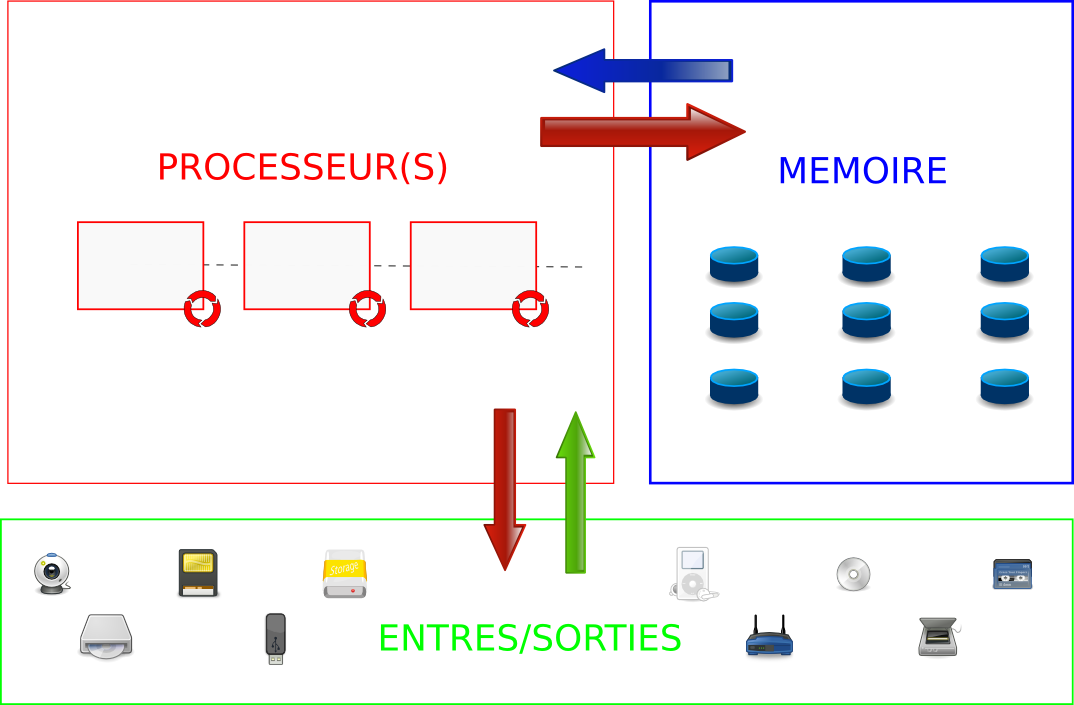
\includegraphics[scale=0.3]{img/cpu-schematics.png}
      \caption{Schéma simplifié du fonctionnement d'un ordinateur}
      \label{schema-ordi}
    \end{center}
  \end{figure}

  \paragraph{} Comme l'illustre le dessin \ref{schema-ordi} (page \pageref{schema-ordi}), un
  ordinateur, aussi complexe soit-il peut être résumé aux trois composants suivants:
  \begin{description}
    \item[Processeur] unité de traitement de l'ordinateur, c'est lui qui réalise les calculs et qui
    produit les résultats ;
    \item[Mémoire] espace de travail du processeur, la mémoire lui permet de stocker les résultats,
    intermédiaires ou finaux, de ses calculs ;
    \item[Entrées/Sorties] pour communiquer avec le "monde extérieur" (clavier, écran, disques durs,
    réseaux,...) le processeur dispose de différents composants matériels dédiés aux différentes
    entrées/sorties.
  \end{description}

  \paragraph{Distinction mémoire vive et mémoire morte} Sans rentrer dans les détails techniques, il
  est important de noter que les périphériques de stockage, tels que les disques durs, ne sont pas
  conceptuellement très différents de la mémoire. Dans les deux cas, ils permettent au processeur de
  stocker des résultats.

  \paragraph{Distinction des types de mémoires} Il existe différents types de mémoires qui peuvent
  être séparées selon qu'elles sont rapide ou lente : plus la mémoire est "proche" du processeur,
  plus elle est rapide. Nous avons donc par ordre décroissant de vitesse :

  \begin{itemize}
    \item la RAM,
    \item le disque dur,
    \item le stockage sur une machine distincte.
  \end{itemize}

  \paragraph{Distinction mémoire vive et mémoire morte}  En outre, il faut noter qu'une mémoire
  \textbf{volatile} a besoin d'électricité pour être conservée, à la différence du \textbf{stockage
  de masse} qui lui conserver l'information une fois l'alimentation coupé. La mémoire volatile est
 donc perdu à chaque arrêt d'un ordinateur alors que les données placées dans la mémoire de masse
 sont conservés..

  \paragraph{} La mémoire vive d'un ordinateur (la "RAM") est une mémoire volatile, et les disques
  dur sont des mémoires de masse.

  \paragraph{} Ce qui sépare donc ces deux composants est leur \textbf{persistance}. L'information
  située en mémoire dite vive (comme la RAM) est \textbf{volatile} : elle disparaît si l'ordinateur s'éteint brusquement. À
  l'inverse, les données placées sur un périphérique de stockage, persiste au delà de l'extinction de
  l'ordinateur.
}

\ifslide{
  \begin{frame}{Qu'est-ce qu'un ordinateur ?}
   \begin{center}
     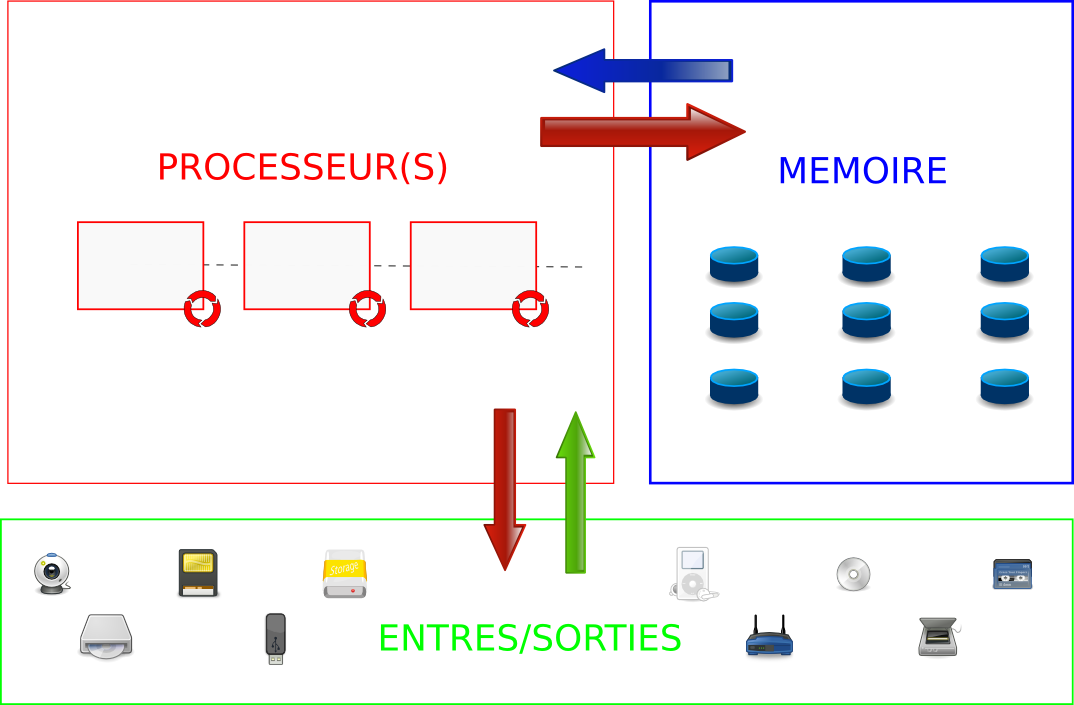
\includegraphics[scale=0.3]{img/cpu-schematics.png}
   \end{center}
  \end{frame}
}

\ifbook{
    \mysubsubsection{Rôle du système d'exploitation}

    \paragraph{} Encore une fois de manière très schématique, et surtout en restant pertinent par
    rapport au thème du cours, le \textit{Middleware}, nous allons maintenant brièvement évoquer le
    rôle du système d'exploitation.

    \paragraph{} En repartant de ce que nous venons de détailler sur le fonctionnement d'un
    ordinateur, plusieurs points peuvent rapidement être gênants. Le principal est que le processeur
    n'exécute qu'un seul programme à la fois, donc tel quel, une seule application peut s'exécuter
    sur un ordinateur à la fois.

    \paragraph{} Le système d'exploitation est une couche logicielle qui va permettre aux programmes
    s'exécutant sur l'ordinateur de se partager les ressources mises à disposition par l'ordinateur
    (processeur, mémoire, périphériques de stockage,...). En outre, le système d'exploitation va
    jouer le rôle d'arbitre entre ces différents programmes, leur attribuant chacun à leur tour un
    certain temps d'utilisation de ces ressources.

    \paragraph{} Ainsi, c'est grâce aux systèmes d'exploitation que de multiples programmes vont
    pouvoir s'exécuter en \textbf{parallèle} sur une machine, qu'elle possède un ou plusieurs
    processeurs.

    \paragraph{} Il est important de noter qu'aucun ordinateur ne pourra effectuer plus de tâches en
    parallèle que son nombre de processeurs, mais les cycles d'exécutions étant extrêmement courts,
    un seul ordinateur, équipé d'un seul processeur, peut donner l'impression à son utilisateur
    d'exécuter simultanément plusieurs tâches. C'est l'impression que vous donne tous les jours,
    les ordinateurs dédiés à la bureautique que vous utilisez.

    \paragraph{Remarque} On notera aussi au passage qu'un même programme peut lui même se diviser en
    plusieurs processus distincts, s'exécutant aussi en parallèle, selon les règles évoquées juste
    avant. Ainsi, dans la cadre d'un projet \textit{middleware} la question de l'exécution, de
    manière concurrente, de différentes parties de l'application peut se poser... (Nous y
    reviendrons plus loin dans le cours).

    \paragraph{} Le schéma \ref{role-os} (page \pageref{role-os} résume les principales
    fonctionnalités d'un système d'exploitation vis-à-vis des applications qui s'exécutent en son
    sein.

    \begin{figure}[h]
      \begin{center}
        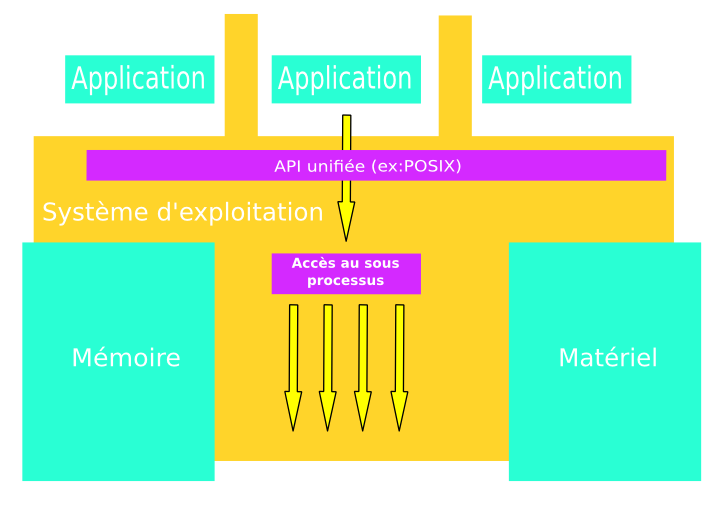
\includegraphics[scale=0.3]{img/operating-system.png}
        \caption{Rôle du système d'exploitation}
        \label{role-os}
      \end{center}
    \end{figure}
}

\ifslide{
  \begin{frame}{Le rôle du système d'exploitation}
    \begin{center}
      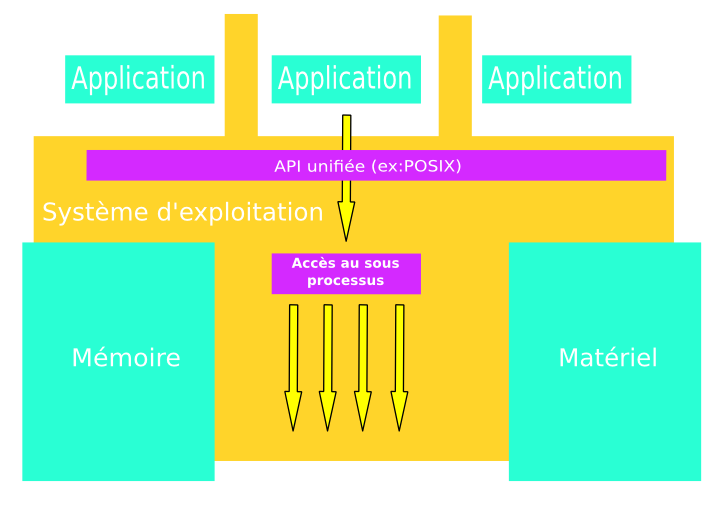
\includegraphics[scale=0.3]{img/operating-system.png}
    \end{center}
  \end{frame}
}

\ifbook{
  \mysubsubsection{Limites physiques d'un ordinateur}
  \paragraph{} Avant d'aller plus loin, arrêtons-nous un instant sur ces notions et sur le système,
  aussi schématique soit-il que nous venons de décrire. Au regard de son fonctionnement, quelles
  limites pouvons-nous déjà percevoir ? Dans quelles conditions, un tel système - l'ordinateur, aura
  des difficultés à effectuer les opérations qu'on lui confie ?

  \paragraph{} Sans surprise, on peut distinguer à peu près autant de limites que de composants
  distingués dans la précédente représentation. Étudions, sommairement, pour chacun d'entre eux les
  limites qu'ils induisent sur l'ordinateur.

  \paragraph{Processeur} La première limite physique d'un ordinateur, qui est pratiquement
  incontournable, est le processeur. Un processeur peut effectuer un certain nombre d'opérations
  dans un certain délai. Dans un système parfaitement optimisé, où tous les autres - assez
  nombreux, nous allons le voir, goulots d'étranglement ont été "neutralisés", cette vitesse
  d'exécution est une limite incompressible : l'ordinateur ne pourra simplement exécuter les
  opérations demandées plus rapidement...

  \paragraph{Parallélisme} Comme évoqué lors de la description du rôle d'un système d'exploitation,
  un ordinateur exécute souvent plusieurs processus à la fois, souvent plus nombreux que son nombre
  de processeurs. Ainsi, il doit passer d'un processus à un autre, à tour de rôle, pour permettre à
  tous de s'exécuter \textit{presque} en parallèle.

  \paragraph{} Il est évident que le passage d'un processus à un autre n'est pas gratuit, et nécessite, de
  la part du système d'exploitation, comme du processeur, un travail supplémentaire qui consiste à
  sauvegarder les données et l'état du processus placé en "pause" et à recharger ceux du processus
  qui "reprend la main".

  \paragraph{} Au bout du compte, si l'ordinateur effectue un nombre de tâches en parallèle
  largement trop grand pour sa capacité, il risque de passer plus de temps à \textbf{changer de
  contexte} entre chaque processus, plutôt qu'à réellement effectuer les opérations qu'on lui
  demande.

  \paragraph{Mémoire} La mémoire à la disposition du processeur impacte généralement grandement la
  vitesse d'exécution. En effet, plus l'ordinateur pourra placer de données en mémoire, plus il
  pourra avoir à sa disposition des résultats intermédiaire et finaux.

  \paragraph{} Illustrons rapidement ce point par un exemple concret. Supposons que l'on confie à
  l'ordinateur de trier un tableau de données, composé d'une seule colonne, par ordre de grandeur
  croissante du contenu de chaque cellule:

  \begin{figure}[h]
    \begin{center}
      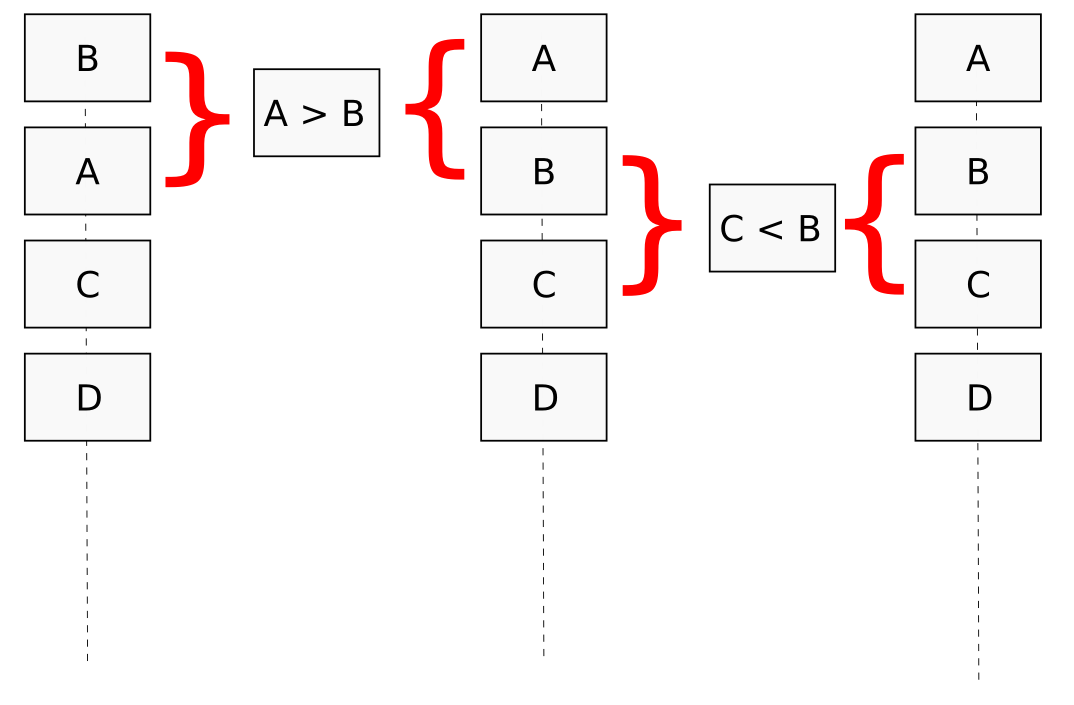
\includegraphics[scale=0.3]{img/exemple-algo.png}
      \caption{Algorithme de tri avec une case mémoire}
      \label{algo-exemple}
    \end{center}
  \end{figure}

}

\ifslide{

  \begin{frame}{Exemple d'algorithme}
    \begin{center}
      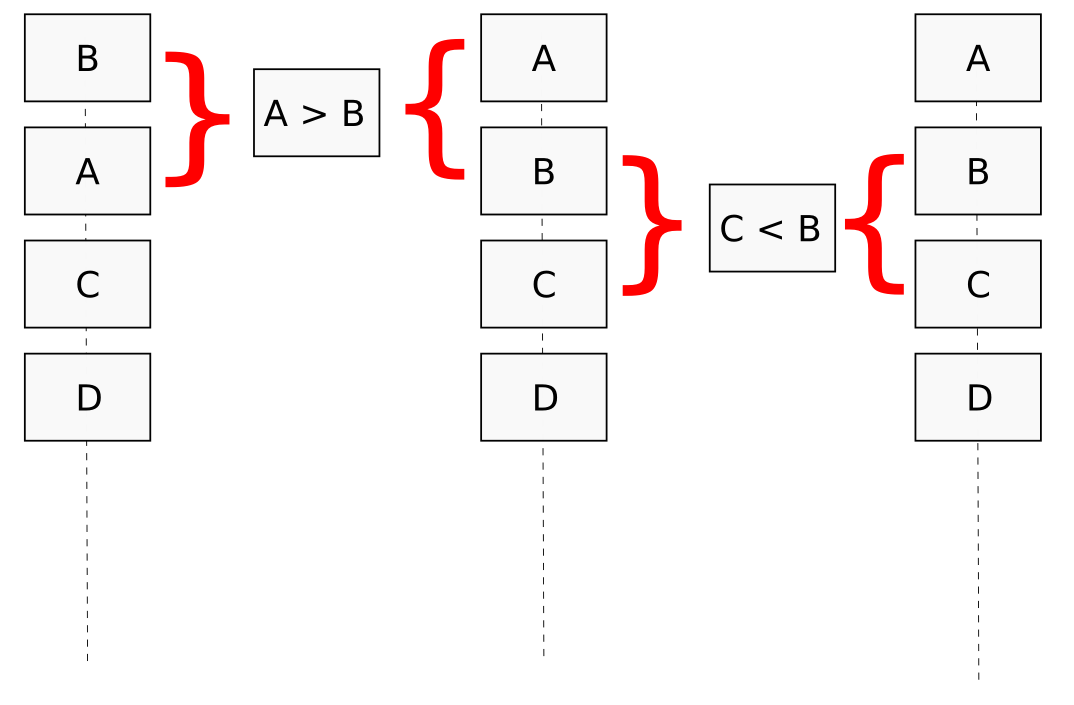
\includegraphics[scale=0.3]{img/exemple-algo.png}
    \end{center}
  \end{frame}
}


\ifbook{

  %TODO:Relire
  \paragraph{} Prenons d'abord comme exemple un ordinateur qui ne pourrait stocker que le contenu
  des quelques cellules du tableau en mémoire rapide. Il devrait alors lire une cellule, lire la
  cellule voisine, les comparer et les réécrire dans le bon ordre. Pour cette opération deux lectures
  et deux écritures ont été nécessaire dans une mémoire lente.

  \paragraph{} Si l'ordinateur avait plus de mémoire alors il aurait pu stocker tout le tableau dans
  sa mémoire la plus rapide, et ainsi réaliser les opérations de lecture beaucoup plus rapidement
  avant d'enfin écrire, en une seule fois, le tableau reclassé dans sa mémoire de stockage de masse,
  elle beaucoup plus lente.

  \paragraph{Remarque} \textit{Cet exemple est volontairement grossier afin de souligner
  l'importance de la mémoire sur la vitesse de traitement.}

  \paragraph{} Si l'ordinateur ne peut stocker qu'un seul résultat intermédiaire, en l'occurrence la
  taille du contenu de la cellule, il ne peut réordonner le tableau qu'en échangeant les cellules
  de positons. En effet, il peut calculer la taille d'une cellule, la stocker, calculer la taille de
  la seconde cellule, la comparer à la précédente et changer l'ordre des deux cellules, si
  nécessaire, puis continuer...

  \paragraph{} Après un laborieux travail, cet \textbf{algorithme}, illustré sur la figure
  \ref{algo-exemple}  (page \pageref{algo-exemple}), sera donc capable de réordonner l'ensemble du
  tableau, mais en effectuant un important nombre d'opérations. À l'inverse, si le processeur est
  libre de placer autant de résultats en mémoire que d'entrées dans le tableau, il pourra se
  contenter de calculer, une fois pour toute, la taille de chaque cellule, puis de les trier de
  manière plus "globale"...

  \paragraph{Remarque} Cet exemple est volontairement très grossier et n'est pas représentatif du
  tout du fonctionnement interne réel d'un ordinateur, ni même de la manière dont le processeur va
  implémenter un algorithme de tri. Néanmoins, sans être l'exemple le plus respectueux des détails
  techniques d'un ordinateur, il illustre de manière très juste l'importance de la mémoire pour la
  réalisation d'opérations au sein d'un ordinateur.

  \paragraph{Entrées/Sorties} Après la mémoire, c'est très certainement les entrées/sorties la
  source de goulot d'étranglement la plus commune au sein d'un ordinateur. Pour bien comprendre
  l'impact de ces dernières sur les performances de l'ordinateur, il suffit de regarder la figure
  \ref{pyramid-io} (page \pageref{pyramid-io} qui décrit, sous forme de pyramide, la vitesse d'accès
  des différentes entrées/sorties, les unes par à rapport aux autres.

  \begin{figure}[h]
    \begin{center}
      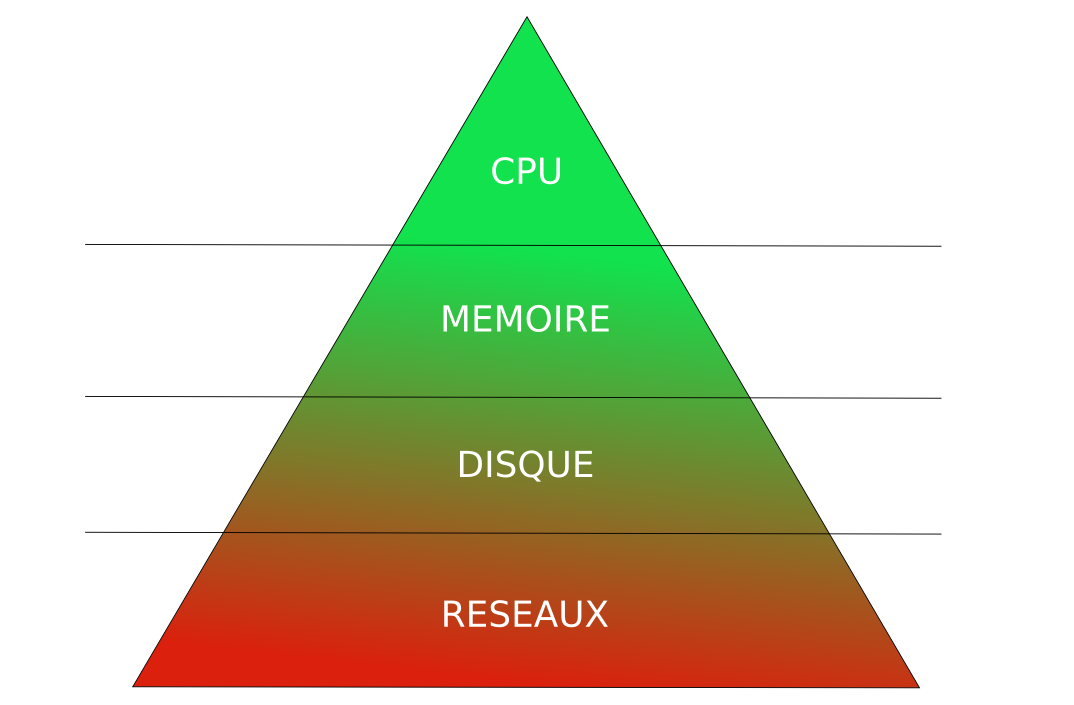
\includegraphics[scale=0.3]{img/pyramid-io.png}
      \caption{Vitesse des entrées/sorties selon les périphériques}
      \label{pyramid-io}
    \end{center}
  \end{figure}

}

\ifslide{
  \begin{frame}{Vitesse d'accès des périphériques}
    \begin{center}
      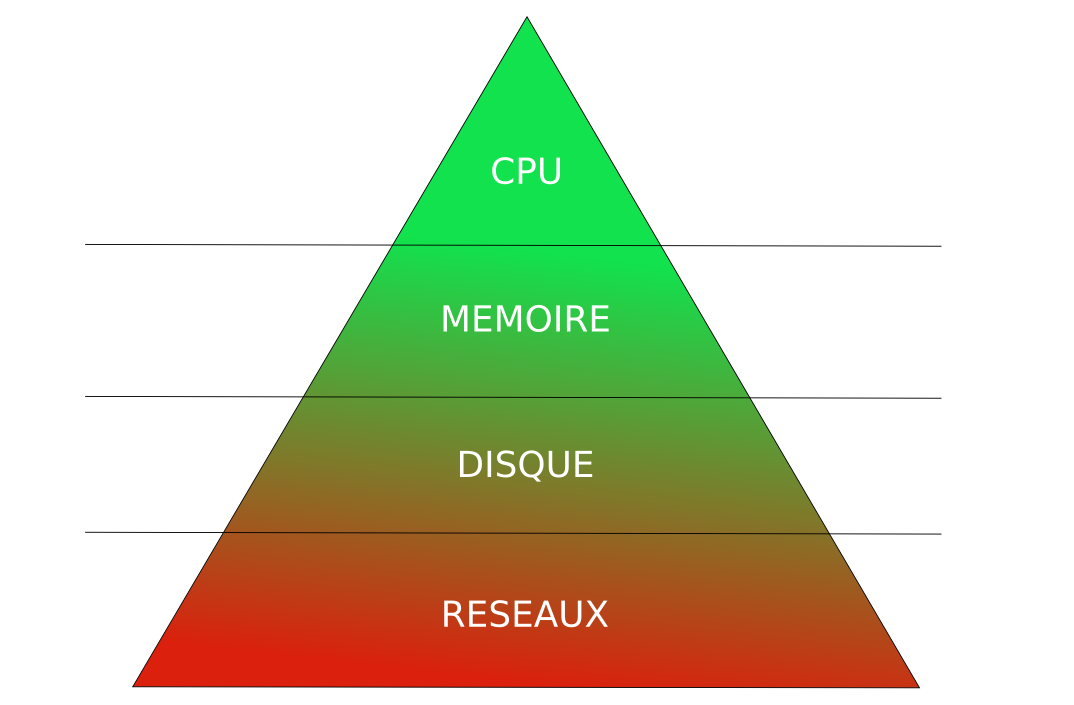
\includegraphics[scale=0.3]{img/pyramid-io.png}
    \end{center}
  \end{frame}
}

\ifbook{

  \paragraph{} À l'étude de ce tableau, il apparaît assez flagrant que si une information nécessaire
  à la bonne exécution du programme est située sur un périphérique inutilement lent (par exemple: sur
  disque dur plutôt qu'en mémoire, sur un serveur distant plutôt que sur le disque dur,...), le
  système en sera ralenti.

  \paragraph{Remarque:} \textit{Ce développement sur les limites physiques d'un ordinateur est volontaire.
  En effet, dans le cadre de la conduite de projet \textit{Middleware}, ces limites seront à
  prendre à compte, dès la conception et l'architecture d'une solution logicielle, pour s'assurer que,
  lors de sa mise en production, le système construit ait une chance de donner les performances
  souhaitées.}

  \paragraph{}\textit{Si des experts techniques sont généralement là pour assister les personnes en charge
  de la conduite, il reste important que ces dernières gardent ses problématiques à l'esprit et soient
  capables d'en discuter avec les susnommés experts...}

}

\subsection{Le modèle client/serveur}

\ifbook{
  \subsubsection{Bref histoire du client léger}
  \paragraph{} Avec l'apparition des réseaux informatiques, apportés par des technologies telles que
  TCP/IP sur laquelle s'est construit le désormais célèbre protocole HTTP, il est rapidement apparu
  très intéressant de pouvoir répartir le traitement sur plusieurs machines.

  \paragraph{} En effet, au début de l'informatique, les machines puissantes coûtaient relativement
  cher, et avaient des capacités de calculs permettant d'effectuer des calculs complexes et de
  répondre aux besoin de nombreux utilisateurs. Ainsi est né le modèle client/serveur, où
  l'utilisateur, à l'aide d'un terminal - une machine peu puissante et peu couteuse, se connecte à
  une machine lui servant des données et exécutant les traitements demandés- un serveur. Le terminal
  se contentant, dans ce modèle, d'afficher le résultat.

  \begin{figure}[h]
    \begin{center}
      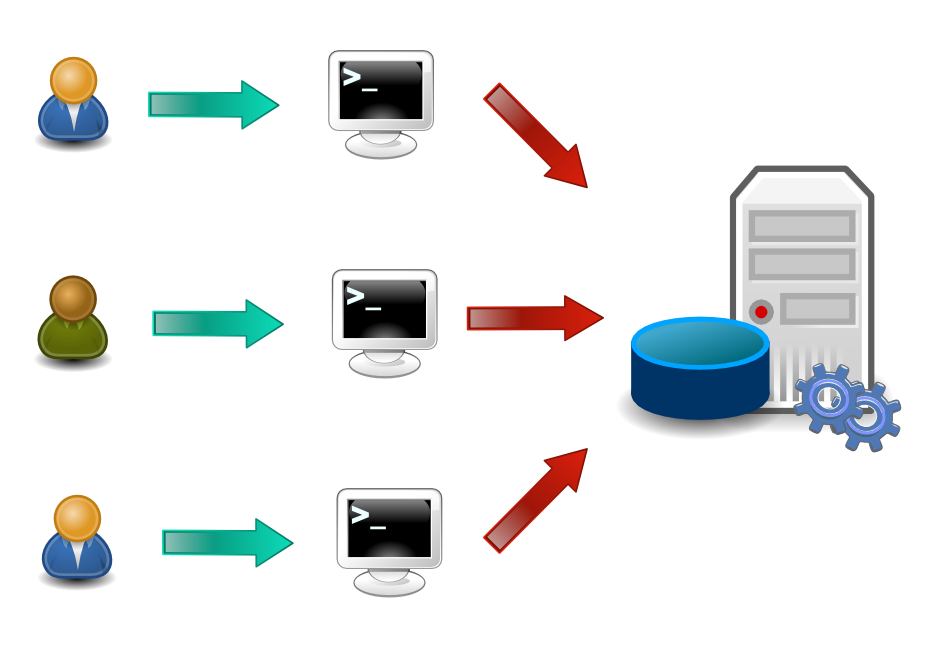
\includegraphics[scale=0.3]{img/mainframe-terminals.png}
      \caption{Terminaux et mainframe}
      \label{mainframe}
    \end{center}
  \end{figure}
}

\ifslide{
  \begin{frame}{Mainframe et terminaux}
    \begin{center}
      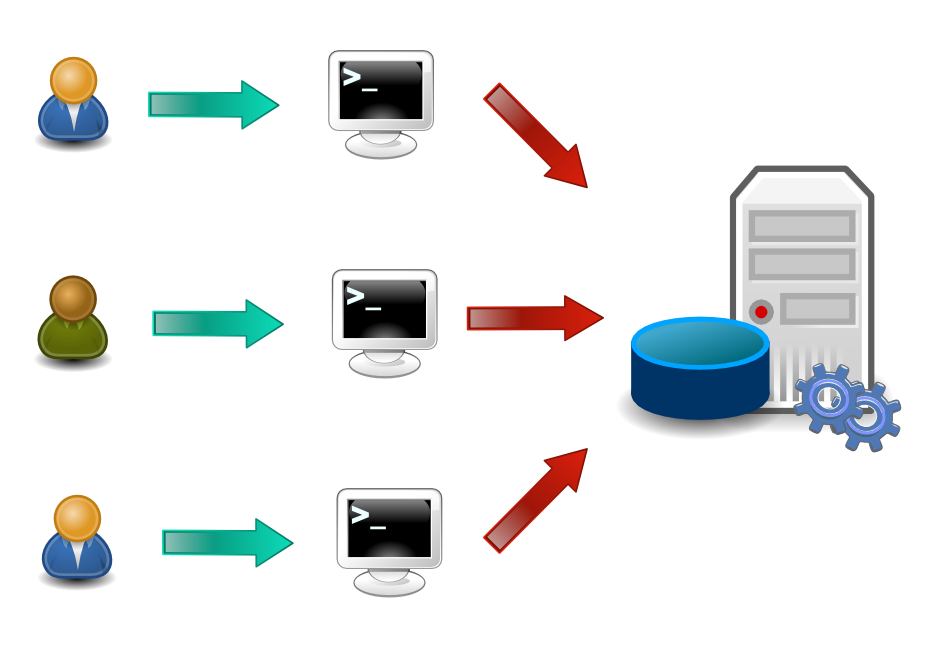
\includegraphics[scale=0.3]{img/mainframe-terminals.png}
    \end{center}
  \end{frame}
}

\ifbook{

  \paragraph{} Avant d'aller plus loin, on peut noter avec intérêt que ce modèle n'est en fin de
  compte pas très différent de celui des débuts d'internet. En effet, à leurs débuts, les
  navigateurs "web" (Mozaic, Netscape, puis Internet Explorer) se contenter simplement d'afficher le
  contenu des pages HTML qu'on leur servaient. Nous y reviendrons par la suite...

  \subsubsection{La naissance du client "lourd"}

  \paragraph{} Ce premier modèle client/serveur se construisait donc sur deux logicielles distincts,
  une première partie s'exécutant sur le terminal de l'utilisateur, le \textbf{client léger}, et une
  seconde partie, plus élaboré et embarquant la \textbf{logique métier} de l'application, le
  \textbf{serveur}.

  \paragraph{Remarque} \textit{L'usage a malheureusement imposé depuis longtemps l'utilisation du même
  terme, \textit{serveur} pour désigner deux entités conceptuellement, mais concrètement
  différentes. Ce terme peut en effet indiquer une machine physique, un ordinateur, relié à un
  réseau informatique et utilisé, à distance, par des utilisateurs, mais le logicielle s'exécutant
  sur ce même type d'ordinateur et fournissant un service applicatfs à ces mêmes utilisateurs.}

  \paragraph{} \textit{La différence est fortement relativement aisée à saisir, mais elle peut tout de même
  porté à confusion. Si dans le cas de la partie précédente nous évoquions la concept de machine
  physique, dans cette section, nous parlons très clairement de \textbf{serveur logicielle}.}

  \paragraph{} Alors que la puissance à la disposition des terminaux augmentaient, et que, dans les
  faits, ceci devinrent des ordinateurs graphiques à usage personnelle ("\textit{Personal Computer
  (PC)}"), il apparu rapidement très pertinent d'en profiter pour offrir des clients plus puissants,
  capable d'effectuer des traitements par eux même, et offrir donc des fonctionnalités
  supplémentaires à leur utilisateurs.

  \paragraph{} Ainsi le mouvement de balancier, qui avait pour but de placer le maximum de logique
  applicatif et de traitement du coté du \textit{serveur}, s'est inversé et les logicielles clients
  devinrent à leur tour de plus en plus complexe, au point qu'on les qualifia de \textbf{clients
  lourds}.

  \begin{figure}[h]
    \begin{center}
      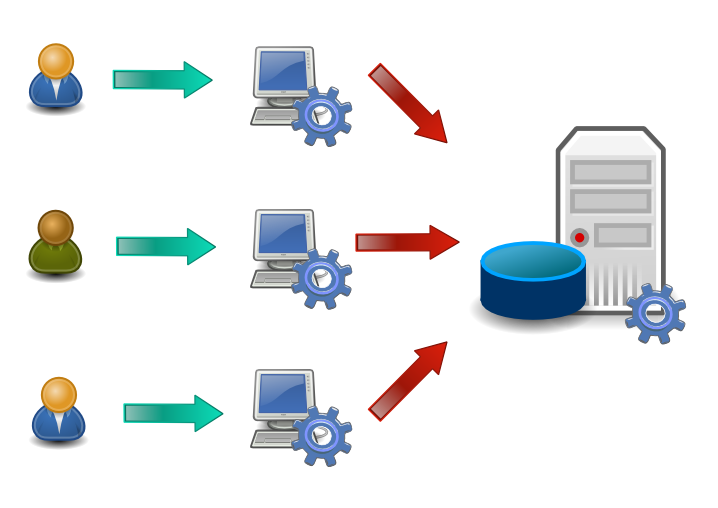
\includegraphics[scale=0.3]{img/fat-clients.png}
      \caption{L'arrivée du PC et des clients lourds}
      \label{fat-clients}
    \end{center}
  \end{figure}

  \subsubsection{Les limites du modèles}

  \paragraph{} Si ce nouvelle déclinaison du modèle aboutit clairement à une manière productivité
  des utilisateurs, du moins dans la plupart des cas, elle posa aussi rapidement des problématiques
  complexes en termes de maintenance. En effet, pour pouvoir faire évoluer le logiciel, il faut
  désormais modifier à la fois le client et à la fois le serveur, et assurer leur rédéploiement
  synchrone. On se retrouva vite malheureusement dans des situations difficiles à gérer, où de
  multiples versions d'une même application clientes sont déployés et doivent cohabiter avec des
  versions différentes de leurs serveurs...
}

\ifslide {
  \begin{frame}{Le modèle client/serveur}
    \begin{center}
      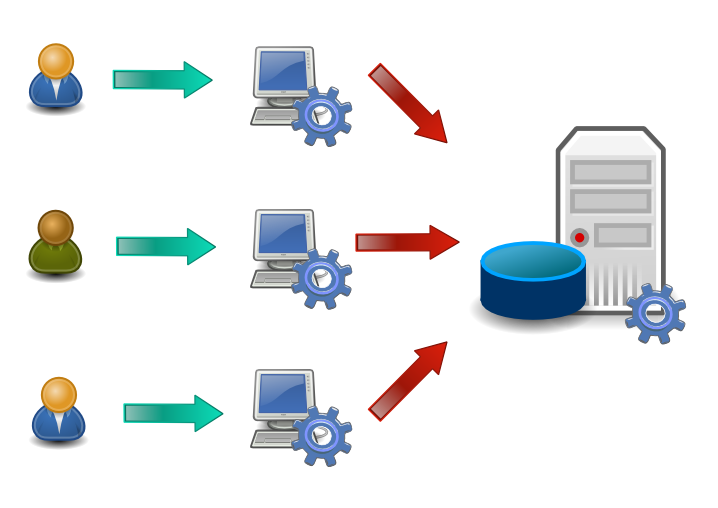
\includegraphics[scale=0.3]{img/fat-clients.png}
    \end{center}
  \end{frame}
}


\ifbook{
  \subsubsection{La Persistance des données: du fichier à la base de données}
  % fichier et répertoires
  \paragraph{} Avant de voir comment les technologies de type client/serveur ont évoluées pour
  circonvenir les problématiques apparues avec l'émergence du client lourd, intéressons nous instant
  non plus au logiciel, mais à ses données, et surtout à leur persistence.

  \paragraph{} Comme évoqué plus haut, un ordinateur travaille avec des données en mémoire et qui
  sont donc par essence, \textbf{volatile}. En effet, lors de l'interruption de l'alimentation de la
  mémoire, les données qu'elle contient sont purement et simplement perdues. Les données n'étant,
  dans la plupart des applications, que rarement dispensable, il a été impératif de trouver des
  mécanismes pour assurer leurs \textbf{persistences}.

  \paragraph{} L'unité atomatique de cette persistence est le \textbf{fichier}. Cette abstraction
  permet de sauvegarder sur une unité de stockage (en langage vernaculaire, un "disque dur") une
  un ensemble d'information de manière séquentielle. On peut retrouver les informations stocké à
  l'aide du nom du fichier.

  \paragraph{} En fait, on peut aisément comparer un fichier à une simple feuille, sur laquelle on
  écrit les données que l'on souhaite persister, un peu de la même manière dont on écrit sur une
  feuille sa liste de courses, pour justement, ne pas l'oublier.

  \paragraph{} Pour permettre de trier et de ranger ses fichiers, dans la prolongation de l'image
  choisi pour les fichiers, des fichiers spéciaux, les \textbf{répertoires} ont été conçu pour
  permettre de aisément ranger et hierarchisé les fichiers.

  \paragraph{} Malheureusement, la manière séquentielle d'organiser les informations d'un fichiers
  se révèla contraignant. En effet, alors que les applications se complexifiaient, et qu'une données
  fit référence à une autre, puis à une autre, la nature \textbf{relationnelle} devint évident et
  imposa un changement de stratégie dans l'approche de leur persistece.

  \paragraph{} En outre, les données nécessite bien souvent d'être partagé entre plusieurs
  applications, et il est fort complexe de partager un fichier de données entre plusieurs
  applicatons. Comment gérer les accès concurrents ? Comment assurer la cohérence des données qui
  sont persisté ?
  % base de donnée
  \paragraph{} Pour palier à ses nombreux problèmes et surtout clairement séparer les données des
  applicatifs, les premières base de données relationelles firent leurs apparitions. En plus de
  permettre de stocker les données hors des applications et de les partager, elles permirent, peu à
  peu, d'établir un langage standard pour interagir avec elles, le SQL (\textit{Standard Query
  Language}).
}

\demoframe{Le SQL}{Argument optionnelle pour le moment}

\ifbook{
  \subsubsection{Architecture n-tiers}
    \paragraph{} Si nous résumons les différents éléments évoqués jusqu'à maintenant sous forme de
    la figure \ref{n-tiers} (page \pageref{n-tiers}), on constate que désormais notre application,
    qui au départ s'exécutait sur une seule machine, relié par un terminal très primaire, est
    désormais réellement éclatée entre plusieurs composant, ou \textbf{tiers}.

    \paragraph{} Ainsi, de l'architecture client/seveur, composé de deux tiers, on est arrivée à une
    architecture 3 tiers, où la base de données vint s'ajouter, en tant que troisième tiers. Mais en
    fait, la séparation des fonctions sur différentes instances physiques a continué, et
    aujourd'hui on parle plus en plus souvent d'architecture \textbf{n-tiers}.

    \begin{figure}[h]
      \begin{center}
        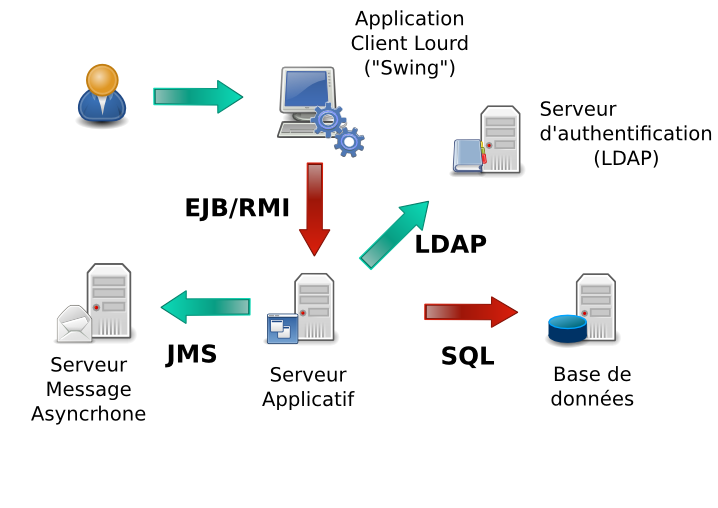
\includegraphics[scale=0.3]{img/n-tiers.png}
        \caption{Exemple d'architecture n-tiers}
        \label{n-tiers}
      \end{center}
    \end{figure}
}

\ifslide{
  \begin{frame}{Architecture n-tiers}
    \begin{center}
      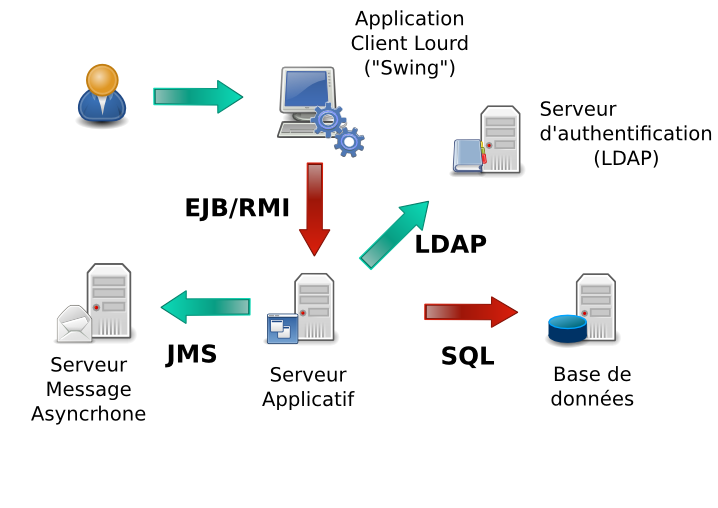
\includegraphics[scale=0.35]{img/n-tiers.png}
    \end{center}
  \end{frame}
}

\ifbook{
  \mysubsubsection{Le Web}
  \paragraph{} Avec l'arrivé des technologies du "Web", soit essentiellement au début, HTML et HTTP,
  le mouvement de balancier évoqué une précédente section s'inverse de nouveau. Dans leurs
  laboratoires, les concepteurs initiale de ce protocole de communication visèrent avant tout la
  simplicitié pour assurer surtout une bonne compatibilité entre les différents systèmes existants
  de part le monde.

  \paragraph{} En effet, avant d'aller plus loin, il est important de se rappeler que à cette
  époque, il existait de nombreux systèmes d'exploitation, tous différents et rarement interopérable
  entre eux. Les plus connues aujourd'hui Apple et Windows, mais à l'époque s'ajouté aussi de
  nombreux types d'Unix différents (cf. \textit{\mylink{http://en.wikipedia.org/wiki/Unix\_wars}{Unix
  Wars}}), accompagné par nombreux autres systèmes, tel que OpenVMS.

  \paragraph{} Sans compter que ces systèmes avaient même des protocoles de communications
  différents. Pour reprendre l'exemple de OpenVMS, ce système utilisé un protocole propriétaire à
  son constructeur, intitulé DecNet et non le standard \textit{de facto} d'aujourd'hui, le protocole
  TCP/IP.

  \paragraph{} Ainsi, concevoir un système applicatif portable - c'est à dire qui fonctionnerait à
  peu près partout et permettrait de communiquer aisément entre des systèmes différents n'était pas
  une simple tâche. C'est donc pour ces raisons, en autres, que les concepteurs de HTTP et de HTML
  ont choisi de faire très simple.

  \paragraph{} Le protocole en lui même est un simple protocole \textbf{texte}, et non binaire, il
  est donc aisé de l'implémenter et, au besoin, de regarder l'échange en lui même pour comprendre la
  source d'un problème. Comme les données échangés sont du texte, tout systèmes de l'époque, aussi
  différent soit-il des autres, était capable de le comprendre.
}

\demoframe{Le protocole HTTP}{
  \begin{block}{Démonstrations}
    \begin{itemize}
      \item simple connection avec telnet
      \item connection complète avec les développeurs tools de Google Chrome
    \end{itemize}
  \end{block}
}

\ifbook{

  \paragraph{} Toujours par souci de simplicité, l'objectif était dans les faits assez peu ambitieux,
  puisqu'il s'agissait d'afficher du contenu simple, du texte un peu enrichi, pour permettre en fait
  au milieu universitaire de publier, facilement et rapidement,  à l'intention de leurs confrères,
  des informations.

  \paragraph{} La conséquence directe de ce choix simple de données utilisés à été de limiter le
  rôle du client à afficher, du mieux possible selon le systèmes utilisées, les informations
  fournies par le serveur HTTP. Le \textbf{client lourd} venait de faire un régime et redevenait un
  \textbf{client léger}.

  % TODO: Dessins de synthèse "web" début
    \begin{figure}[h]
      \begin{center}
        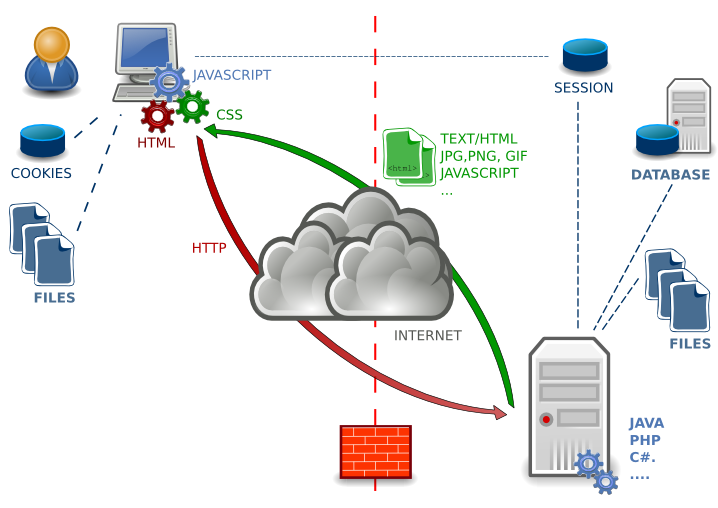
\includegraphics[scale=0.3]{img/internet.png}
        \caption{Extrait de code HTML contenant du Javascript et du CSS}
        \label{internet}
      \end{center}
    \end{figure}
}

\ifslide {
    \begin{frame}{Le "Web"}
      \begin{center}
        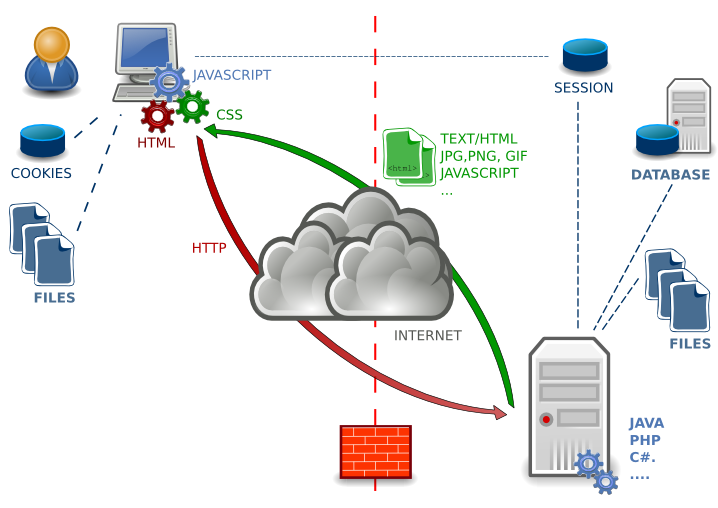
\includegraphics[scale=0.3]{img/internet.png}
      \end{center}
    \end{frame}
}

\ifbook{
  \mysubsubsection{Les technologies "Web" s'enrichissent}
  % Formulaire et session HTTP
  \paragraph{} Le protocole HTTP, et son format de donnée, HTML, a eu le succès qu'on connait, et
  rapidement, malgré l'élégance de la simplicité de la solution, il apparu clair que d'\textbf{absence
  d'interfaction} entre l'utilisateur et le serveur HTTP était une limite trop contraignante. En
  effet, tel que nous l'avons évoqué jusqu'à maintenant, le modèle ne permet en essence que de
  télécharger un page au contenu \textbf{statique}.

  \paragraph{} Pour introduire plus d'interactivité, et permettre au serveur HTTP de modifier
  \textbf{dynamiquement} le contenu des pages présentées selon les demandes des utilisateurs, les
  formulaires ont été introduit. Ces derniers, associés à la méthode HTTP POST, ont donc permis aux
  utilisateurs d'envoyer des données au serveur HTTP, qui furent le point de départ des premières
  applications "web".

  \paragraph{} Mais une fois qu'il fût possible d'envoyer ces données, d'autres limites firent leur
  irruptions. La plupart des applications nécessitant souvent plusieurs échanges entre l'utilisateur
  et le serveur, il fût nécessaire d'ajouter un mécanisme de son coté pour lui permettre de
  conserver les données associées à l'utilisateur, ou plutôt à sa \textbf{session}.

% TODO:Cookies ?
%  \paragraph{} L'ajout donc de la notion de session HTTP permit, là encore, de contourner les limites
%  du modèle original, mais elle ne suffit pas entièrement. De la même manière dont le serveur avait
%  besoin de garder trace de son utilisateur, il fallait aussi que l'on soit en mesure, coté client,
%  de conserver une trace.

  % CSS et Javascript
  \paragraph{} Alors que la première génération de site web finissaient de fleurir, une
  problématique, jusque là invisible, apparu de plus en plus clairement. Le HTML, dans toute la
  beauté de sa simplicité, enfreint par son essence même, une règle pourtant fondamentale de
  l'informatique, que nous avons déjà évoqué avec les bases données : la séparation du contenu et de
  sa présentation.

  \begin{figure}[h]
    \begin{center}
      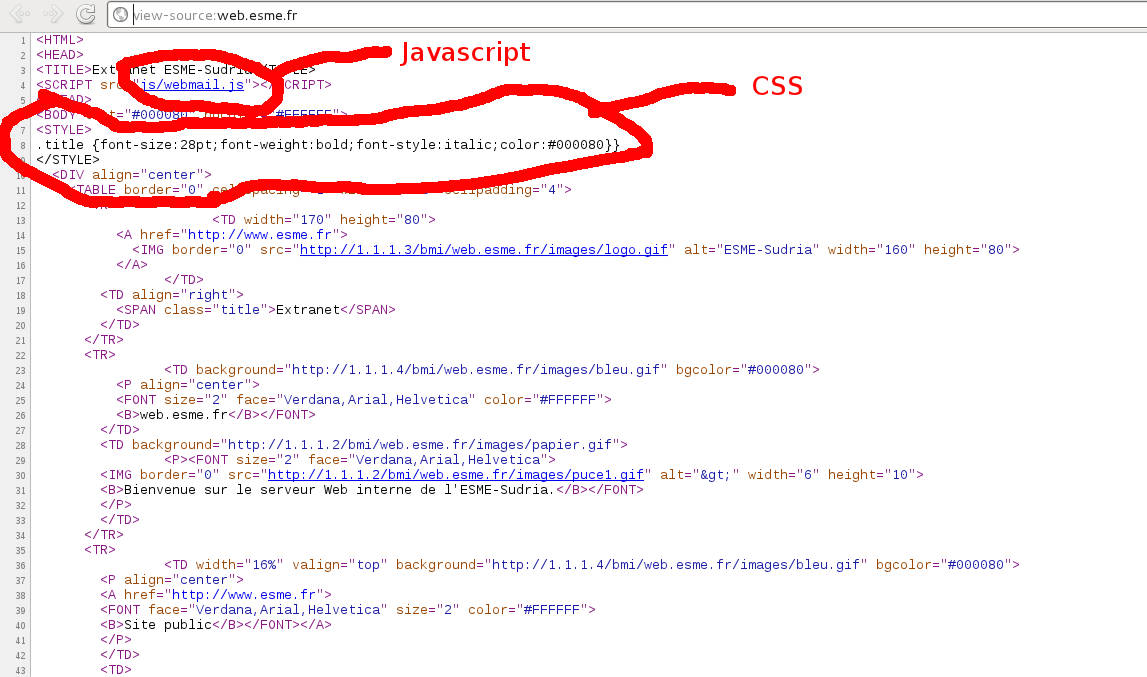
\includegraphics[scale=0.3]{img/html-code-sample.png}
      \caption{Extrait de code HTML contenant du Javascript et du CSS}
      \label{middleware}
    \end{center}
  \end{figure}
}


\ifslide {
  \begin{frame}{HTML, CSS et JavaScript}
    \begin{center}
      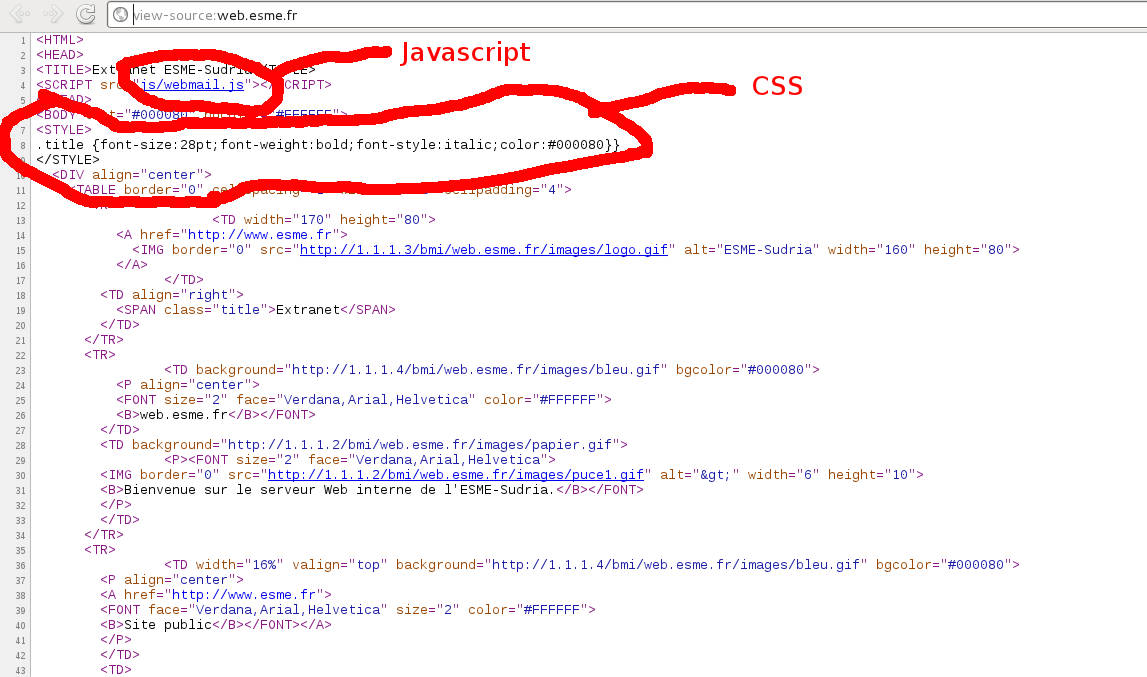
\includegraphics[scale=0.3]{img/html-code-sample.png}
    \end{center}
  \end{frame}
}

\ifbook{
  \paragraph{} En effet, au sein d'une page HTML, on mélange avec allégresse texte avec sa
  présentation qu'il s'agisse de le mettre en gras ou ialic, ou bien de le positionner au sein de la
  page. Et cet état fait rendu rapidement très difficile de faire évoluer, du point fonctionnel, les sites -
  puisque les graphistes ou ergonomes ne pouvait pas travailler de manière indépendantes des
  programmeurs, mais aussi de faire évoluer leurs chartes graphiques, puisque leurs simples mise à
  jour nécessitant de modifier l'intégralité des pages...

  \paragraph{} C'est ainsi que est apparu le CSS, \textit{Cascading Style Sheet}, ou plus
  simplement, les feuilles de styles, dont l'objectif était non seulement de permettre de modifier
  la présentation d'une page HTML existante, mais aussi de séparer la partie présentation d'un site,
  de ses données.

  \paragraph{} En parallèle à l'utilisation du CSS, un autre langage a été introduit, sous forme de
  script, placés dans la page, mais dont l'exécution est déclencheur par le navigareur et qui donc
  fonctionne non plus le serveur, mais sur l poste client.

  \paragraph{} Introduit tout d'abord de manière propriétaire, ce petit langage permis de rendre les
  sites "web" tellement plus dynamique et \textbf{conviviale}, en améliorant grandement
  l'interfaction de l'utilisateur avec ces dernirs, qu'il fût rapidement adopté, et même normalisé
  sous le nom, rarement utilisé, de ECMAScript.
}

\ifbook {
  \mysubsubsection{Conteneur d'exéctution d'application "web"}
  \paragraph{} Comme nous l'avons brièvement résumé, les technologies du "web" se sont construites
  sur une forte volonté d'offrir un système ouvert, standard et interopérable. À l'aide des
  abstractions choisi, et du modèle relativement simple, une page HTML, aussi complexe soit-elle,
  peut être rendu - à peu près, de manière similaire, quelques soit le système d'exploitation
  utilisé.

  \paragraph{} Mais, du coté serveur, les technologies étaient toujours très \textbf{adhérente} à ce
  dernier. Que vous exécutiez sur Apache HTTP, à l'aide du mod CGI, des scripts Shell sous Unix, ou
  que vous écriviez des pages ASP sur un serveur Microsoft, le code réalisé restait indéniablement
  spécifique à son cadre d'exécution.

  \paragraph{} Progressivement, un certain nombres de cadre d'exécution (et de dévelopements)
  d'application "web" virent le jour, tel que PHP et Java. Ces deux derniers, pour continuer avec
  eux, forment des langages de programmation à part entière, mais le modèle qu'ils proposent apporte
  surtout une réelle interopérabilité coté serveur.

  \paragraph{} En effet, avec ce genre de technologie, il devint possible d'exécuter son programme
  sur n'importe quel type de serveur avec un comportement (presque) identique. On pu donc enfin
  aisément migrer de systèmes d'exploitation, dans le cas où celui ci ne se comporte pas de manière
  suffisante pour l'application, ou recruter un développeur sans que celui ci n'est besoin d'autre
  compétences que la seule maitrise de la technologie.

  \paragraph{} En outre, ces technologies promeuvent, pour la plupart, un certain \textbf{modèle de
  programmation}, et l'ecosystème qui les entourent apportent son lot de composants prêt à utiliser
  et destiné à faciliter le développement d'application robuste et capable de monter en charge.

  \begin{figure}[h]
    \begin{center}
      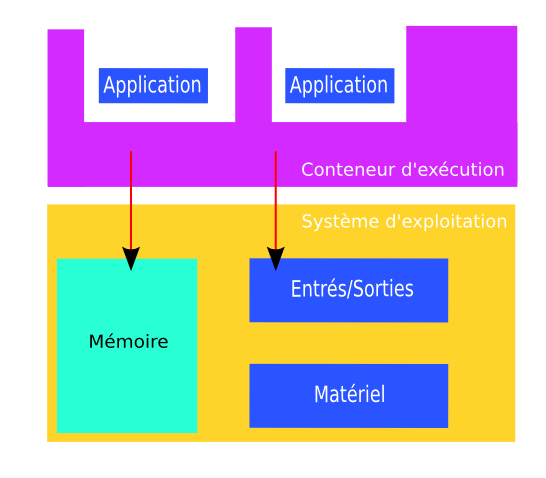
\includegraphics[scale=0.3]{img/execution-container.png}
      \caption{Rôle d'un conteneur d'exécution}
      \label{execution-container}
    \end{center}
  \end{figure}
}


\ifslide {
  \begin{frame}{Conteneur d'exécution}
    \begin{center}
      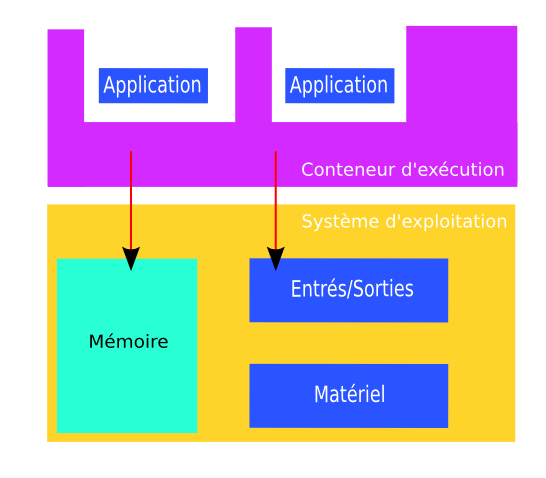
\includegraphics[scale=0.3]{img/execution-container.png}
    \end{center}
  \end{frame}
}

\subsection{Qu'est ce que le middleware ?}

\ifbook {
  \paragraph{} Après ce vaste état des lieux, nous allons enfin pouvoir rentrer dans le thème de ce
  cour: le \textit{Middleware}. En premier lieu, essayons de trouver une définition un plus parlante
  de ce terme, qui n'est pas réellement de traduction française.

  \paragraph{} Si on on traduit très littéralement ce terme, on obtient quelques chose de l'ordre du
  "matériel du milieu". Bon, c'est peu parlant, mais clairement le suffix "\textit{-ware}" fait echo
  aux termes \textit{"software"} - le matériel logiciel, et \textit{"hardware"}, le matériel
  physique, ce qui signifie que, en fait, le mot clé ici, est le "milieu".

  \paragraph{} Mais de quoi exactement sommes nous au milieu ici ? Revoyons simplement notre dessin
  d'architecture à n-tiers:

  \begin{figure}[h]
    \begin{center}
      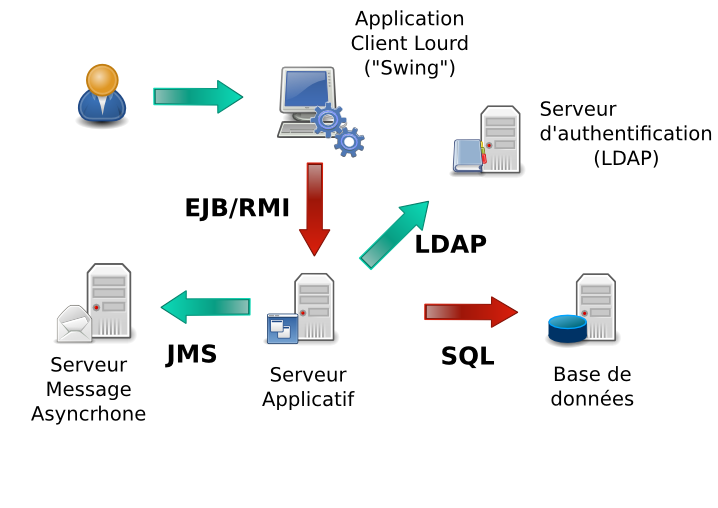
\includegraphics[scale=0.3]{img/n-tiers.png}
      \caption{Où se trouve le middleware sur cette figure ?}
      \label{where-is-middleware}
    \end{center}
  \end{figure}
}

\ifslide{
   \begin{frame}{Qu'est ce que le middleware ?}
     \begin{center}
       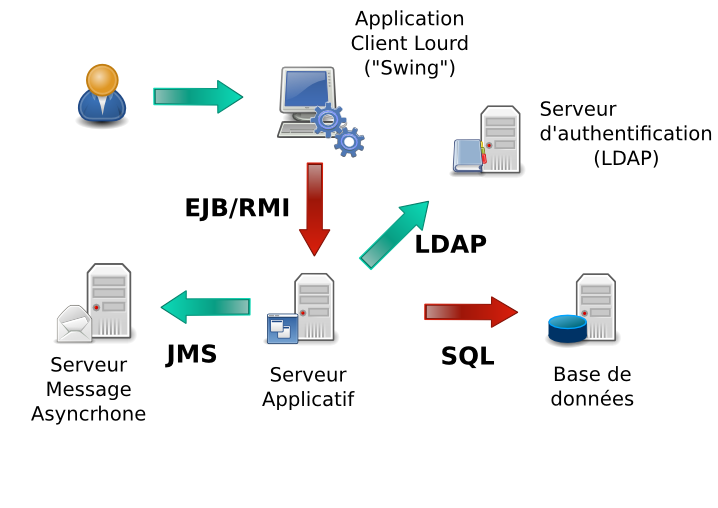
\includegraphics[scale=0.35]{img/n-tiers.png}
     \end{center}
   \end{frame}
}

\ifbook{

  \paragraph{} Le \textit{Middleware} est tout simplement ce qui se retrouve, littéralement, au
  milieu ! Soit entre la base de données et les clients utilisées par les usagers du système. Mais
  au milieu, il y a l'application, non ? Certes oui, mais, celle ci ne s'appuye désormais plus sur les
  seules API fournies par le système d'exploitation, mais sur une kyrielle de services. Ces derniers
  proviennent soit de son environnement d'exécution - tel que une machine virtuelle comme celle de
  Java ou C\#, ou un serveur d'application, ou encore par des composants que l'application elle-même
  embarque.

  \paragraph{} Mais qu'apportent ces services de plus ? Nous allons étudier le "catalogue" en
  détails durant ce cours, mais en quelques mots, ils apportent beaucoup ! Gestion de \textit{pool}
  de connexion, cache locale ou distribué, sécurité, intégration avec un service d'authentification
  distant ou même encore la capacité de mettre en \textit{cluster} l'application pour assurer
  aisément sa montée en charge simplement en ajoutant de nouvelles machines.

  \paragraph{} Pour en revenir à une sorte de définition du \textit{Middleware}, nous retiendrons
  donc que ce dernier est l'ensemble des services utilisées par l'application, aussi bien en son
  sein, que pour communiquer avec des services distants. Bref, en essence, le \textit{Middleware} se
  trouve bel et bien "au milieu", entre l'application et le reste du monde...

  \paragraph{} En essence, le \textit{Middleware}, c'est les briques avec lesquelles on construit
  l'application métier que l'on souhaite réaliser.
  % TODO: dessin fin de déf du middleware ? (img rigolote ?)
}

\subsection{Caractéristiques de la Programmation Orienté Objet}

\newcommand{\bizProcessExemple}[0]{
  \begin{enumerate}
    \item créer un nouveau salarié dans la base de données
    \item ajouter la salarié dans l'équipe de son manager
    \item notifier par email les membres de l'équipe de l'arrivée du nouveau membre
  \end{enumerate}
}

\ifbook{

  \paragraph{} La paradigme de la programmation orienté objet se retrouve dans  plusieurs
  problématiques liées au \textbf{Middleware}, il est important d'expliciter quelques unes de ses
  caractéristiques.

  \subsubsection{Programmation impérative}

  \paragraph{} La paradigme de la programmation orienté objet se retrouve dans  plusieurs
  problématiques liées au \textbf{Middleware}, il est important d'expliciter quelques unes de ses
  caractéristiques.

  \paragraph{} En premier lieu, il faut savoir que la programmation orienté object se définit
  essentiellement par sa distinction avec la programmation \textbf{procédurale} ou
  \textbf{impérative}. Dans ce style de programmation, on effectue les traitements les uns à la suite
  des autres, en regroupant le code commun dans des fonctions.

  \paragraph{} Prenons l'exemple de traitement procédurale:

  \bizProcessExemple

  \paragraph{} Une approche impérative consisterait ici à réaliser un programme réalisant chacune de
  ces actions, dans l'ordres. C'est une approche tout à fait valide et elle ne pose pas, en soi, de
  problème.

  \subsubsection{Approche par "objet"}

  \paragraph{} Néanmoins, la programmation orienté objet propose une approche, qui apporte de nombreux
  avantages. Cette approche consiste à ne plus se concentrer sur la séquence de traitement à réaliser,
  mais plutôt sur les données utilisées.

  \paragraph{} En effet, le but du jeu ici est d'\textbf{encapsuler} les données dans des objets, et
  ne le laisse le reste du programme interagir avec ces données que par le biais des fonctions
  qu'elles proposent. Ces fonctiones se nomment en fait désormais des \textbf{méthodes}.

  \paragraph{} L'objectif de ceci est de \textbf{masquer} la nature réelle des données, et de
  n'exposer que les traitements disponibles autour de ces données. Ainsi, si la nature des données ou
  même des détails d'implémentations des traitements proposés venaient à changer, ces modifications
  seront transparente pour le reste du programme.
}

\ifslide {
  \subsection{Programmation impérative versus programmation orienté objet}
  \begin{frame}
    \begin{block}{Ajout d'un nouvel employé}
      \bizProcessExemple
    \end{block}
    \begin{center}
      
\includegraphics[scale=0.30]{img/biz-process-banner.png}
    \end{center}
  \end{frame}
}

\ifbook{

  \paragraph{} Illustrons ce point en reprenant notre exemple précédent. Pour implémenter notre
  processus métier - l'ajout d'un nouveau employé dans une équipe, nous allons désormais définir
  plusieurs \textbf{objet}.

  \paragraph{} Le premier objet sera l'objet salarié. Ce dernier résultura de la création du salarié
  dans la base de données de l'entreprise, et il regroupe l'ensemble des données relatives à un
  employé. L'accès à la base de données des salariés sera aussi un objet.

  \paragraph{} Le second objet sera en fait une collection de salarié que forme son équipe. Pour
  réaliser le second point de notre traitement, il suffira donc d'ajouter le salarié créée juste avant
  à la liste des salariés composant l'équipe.

  \paragraph{} Un autre objet sera en charge de l'envoi des mails, et sera donc utilisé pour notifier
  les différents membres de l'équipe de l'arrivée du nouveau membre de l'équipe.
}

\ifslide{
  \begin{frame}
    \begin{center}
      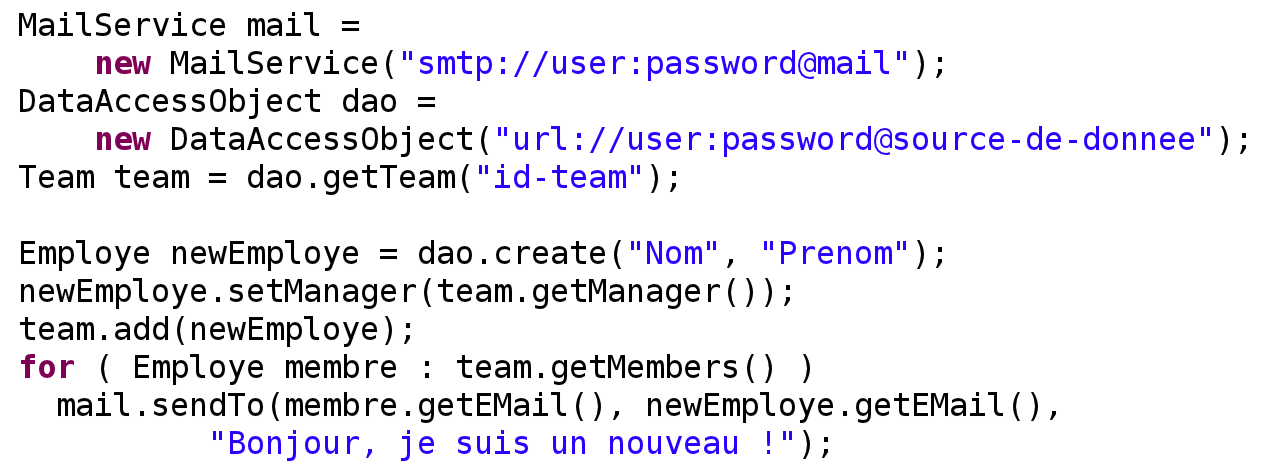
\includegraphics[scale=0.25]{img/biz-process-code-sample.png}
    \end{center}
  \end{frame}
}

\ifbook{

  \begin{figure}[h]
    \begin{center}
      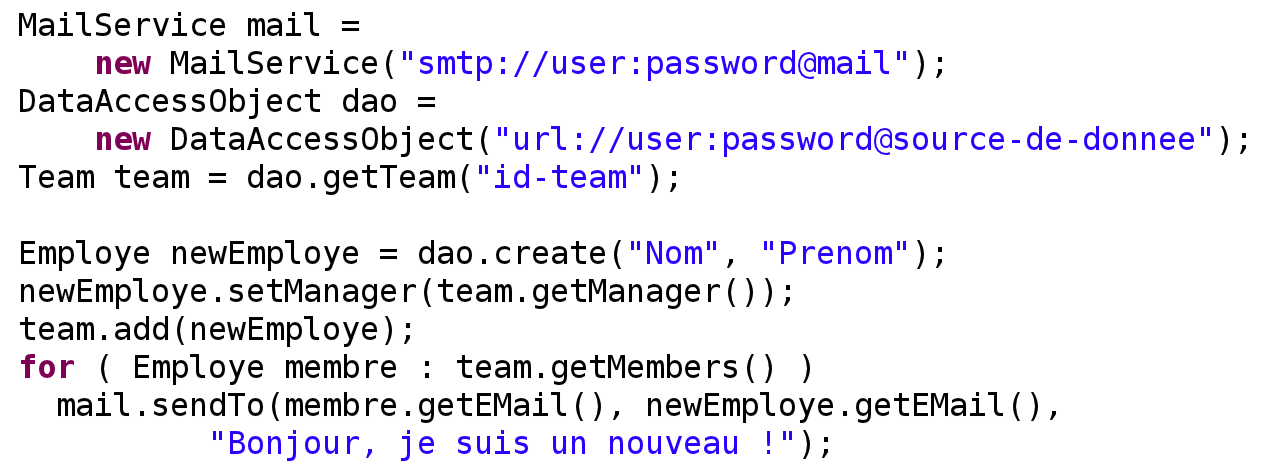
\includegraphics[scale=0.35]{img/biz-process-code-sample.png}
      \caption{Exemple de code orienté objet}
      \label{biz-process-code}
    \end{center}
  \end{figure}

  \paragraph{} Comme l'illustre l'extrait de code \ref{biz-process-code} (page
  \pageref{biz-process-code}, ce style de programmation qu'est la  programmation orienté objet
  permet d'obtenir un code très simple et lisible, mais surtout facilement réutilisable. Par
  exemple, l'objet DataAccessObject regroupe tout le code nécessaire pour se connecter à la base de
  données. Il suffit de réutiliser cet objet, ailleurs dans le code du programme si l'on souhaite
  effectuer des opérations avec la base de données.

  \paragraph{} Un autre avantage immédiat de cette approche est de pouvoir concevoir aisément des
  objets "métiers" décrivant de manière isolé et unitaire, les différents traitements spécifique au
  métier de l'entreprise ou l'organisation. Les différents applications pourront ensuite aisément
  s'appuyer sur ces bibliothèques d'objets pour réaliser les différents traitements qui leur sont
  spécifiques.
}

%- dessin "application" => "pile, gestion de threads, cache, ...", puis vers le modèle java/jee de container
%- évoqué la problématique du packaging et de la réutilisation de code, probablématique de gestion de version aussi

% expliciter/décrire le besoin, dans la conception d'un IT, de découper son "business" en module,
% d'avoir est du code partagé (des Jars) mais aussi des applicatifs qui utilisent les mêmes briques,
% les mêmes services, etc...

\ifslide{
    \begin{frame}{Les Outils des projets informatique}
  \begin{itemize}
    \item Compilation et \textit{build}
    \item Environment de développement IDE (Eclipse)
    \item Gestionnaire de Sources (SVN)
    \item Suivi de tâche (JIRA)
  \end{itemize}
\end{frame}

}

\mysection{B - Les services applicatifs} % 1/2 (10/01/2012)}

\abstractframe{Ciblé sur application, ce chapitre du cours se concentre
sur les services et composants proposés par les \textit{middlewares} à cette
dernière}{../img/overview-services.png}

\ifbook {
  \mysubsection{Remarque préliminaires}
  \paragraph{} \textit{Le champ d'expertise de l'auteur de ce document est Java/JEE, et plus spécifiquement,
  les produits JBoss. Cet état de fait n'est pas sans conséquence sur le contenu du cours, qui
  s'appuie souvent des composants logiciels spécifiques à Java.}

  \paragraph{} \textit{Ainsi, bien que la plupart des concepts évoqués dans cette partie se retrouvent
  généralement, sous une forme ou une autre, dans d'autres univers technologiques, certains seront
  néanmoins parfois relativement spécifiques à l'univers Java ou au monde JBoss.}

  \paragraph{} \textit{Dans la mesure du possible, lorsque ces cas seront évoqués, leur spécifitées sera
  soulignées. Le lecteur devra tout de même rester vigilant...}

}

\mysubsection{Conteneur d'exécution virtuelle}

\ifbook {
  \mysubsubsection{Difficultés des applications natives}

  \paragraph{} Reprenons là où nous avons arrêté, dans la section précédente, la description d'un
  serveur. Nous avions donc une machine physique ou virtuelle dont les ressources (mémoire,
  entrées/sorties, processeurs) sont partagées par l'intermédiaire du système d'exploitation, qui joue
  le rôle d'arbitre entre les différentes applications.

  \paragraph{} Si ce modèle fonctionne très bien, et de nombreuses applications très efficaces ont été
  réalisées sans couche d'abstraction supplémentaire, il pose néanmoins quelques problèmes. Tout
  d'abord, même si l'application utilise le système d'exploitation pour manipuler ressources et sous
  processus, son exécution peut toujours mettre en péril le bon fonctionnement de l'ensemble du
  système.

  \paragraph{} En effet, une application \textbf{native} - qui signifie, dans notre contexte, qu'elle
  n'utilise que les primitives offertes par le système d'exploitation, peut toujours rendre le système
  inopérant en allouant trop de mémoire, en créant trop de sous processus ou encore en écrivant
  beaucoup trop de données sur disque.

  \paragraph{} En outre, si les primitives offertes par le système d'exploitation permet au
  développeur de facilement allouer de la mémoire pour son programme, il reste à sa charge de
  s'assurer que cette espace mémoire soit bien libéré dès qu'il n'est plus utilisé.

  \paragraph{} De prime abord, ceci peut sembler trivial, mais c'est en fait très complexe, et
  beaucoup de programme native ont souvent des \textbf{fuites mémoires} qui pose de grave problèmes
  de performance lors de l'exécution du programme, ou qui, pire encore, entraîne le \textit{crash} du
  programme lors de son utilisation.

  \paragraph{} Mais comment se font ces fuites mémoires ? Simplement lorsque le ou les développeurs
  ont oublié, quelque part au sein de l'application, de libérer des ressources. Ainsi, la mémoire reste
  alloué, tout le temps, et plus le programme s'exécute, plus il "bloque" de la mémoire, jusqu'à atteindre
  un point où le système d'exploitation ne lui permet plus d'en allouer de nouveau.

}

\ifslide{

  \myvertsplitslide{Pourquoi ne plus développer en langage natif ?}{
    \begin{center}
      \begin{itemize}
        \item API bas niveau
        \item Fuite mémoire
        \item Sécurité
      \end{itemize}
    \end{center}
  }{
    \begin{center}
     
\includegraphics[scale=0.25]{img/native-amerindians.jpg}
     \myphotocredit{http://www.flickr.com/photos/37100995@N07/5322106167/sizes/l/in/photostream/}{daniellelorenz}
    \end{center}
}

%  \begin{frame}{Pourquoi ne plus en langage natif ?}
%   \begin{center}
%     \begin{itemize}
%       \item API bas niveau
%       \item Fuite mémoire
%     \end{itemize}
%     
\includegraphics[scale=0.3]{img/native-amerindians.jpg}
%   \end{center}
%  \end{frame}
}

\ifslide{
  \begin{frame}{Garbage collection}
   \begin{center}
     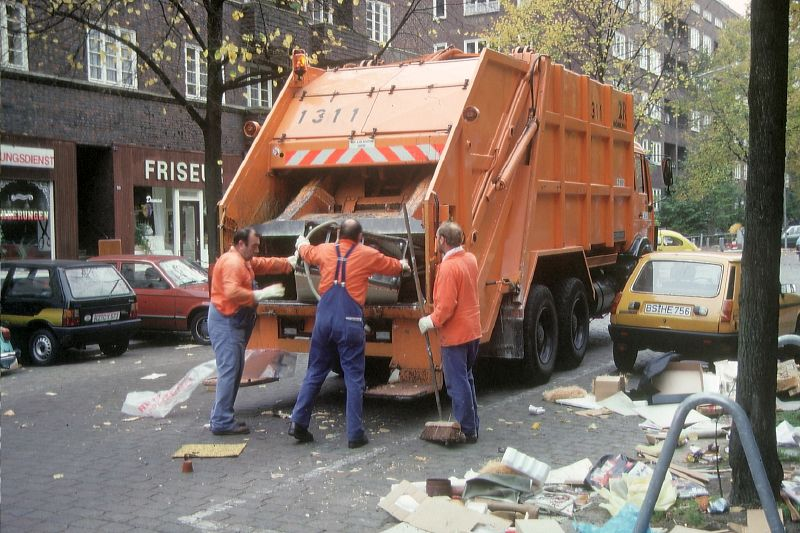
\includegraphics[scale=0.3]{img/garbage-collection.jpg}
   \end{center}
  \end{frame}
}

\ifbook{
  \mysubsubsection{"Garbage collection"}

  \paragraph{} Rapidement la gestion de la mémoire est devenue un tel frein au développement
  d'application, que de nombreuses recherches et expérimentations ont été entreprises pour construire
  une sorte de "méta application" qui assurerait la libération de la mémoire, simplifiant ainsi
  grandement la charge du développeur.

  \paragraph{} Ce \textbf{conteneur d'exécution\footnote{Le terme \textbf{conteneur d'exécution
  virtuelle} est une traduction somme toute très personnelle du terme anglais \textit{runtime
  container}. L'usage a imposé de désigne ce genre de container par leur nom (ex: JVM), plutôt que par
  un terme générique, comme système d'exploitation.}} se charge donc de garder la trace de toutes
  allocations mémoires, mais aussi du nombre de référence vers ces dernières. Lorsque il n'existe
  plus, au sein, du programme, de référence vers un espace mémoire allouée, il ne reste plus qu'à
  faire le \textbf{nettoyage}. En anglais, on emploie fréquemment le terme de \textit{\textbf{Garbage
  Collection}}.

  \mysubsubsubsection{Libération de la mémoire}

  \paragraph{} Comme toujours la création de ce nouveau \textbf{contexte d'exécution} a aussi été une
  opportunité d'introduire une nouvelle couche d'abstraction permettant au programme de se détacher du
  système d'exploitation.

  \paragraph{} Ainsi, on ne développe plus un programme à l'aide des primitives offertes par tel ou
  tel système d'exploitation, mais à l'aide de celles offertes par son conteneur d'exécution. Charge à
  ce conteneur de s'assurer du fonctionnement idoine de ces primitives quelques soit le système
  d'exploitation sur lequel il s'exécute.

  \mysubsubsection{Quelques conteneurs d'exécution}

  \paragraph{} La machine virtuelle Java est un exemple de tel conteneur d'exécution, mais aussi
  l'interpréteur python ou PHP. Ces différents programmes exécutent un code, qu'il soit compilé ou non
  avant\footnote{C'est d'ailleurs cette seule notion de code compilé ou interprété qui distingue
  principalement la machine virtuelle Java des interpréteurs comme Python}, en abstrayant le système
  d'exploitation sous jacent.

  \begin{figure}[hb]
    \begin{center}
      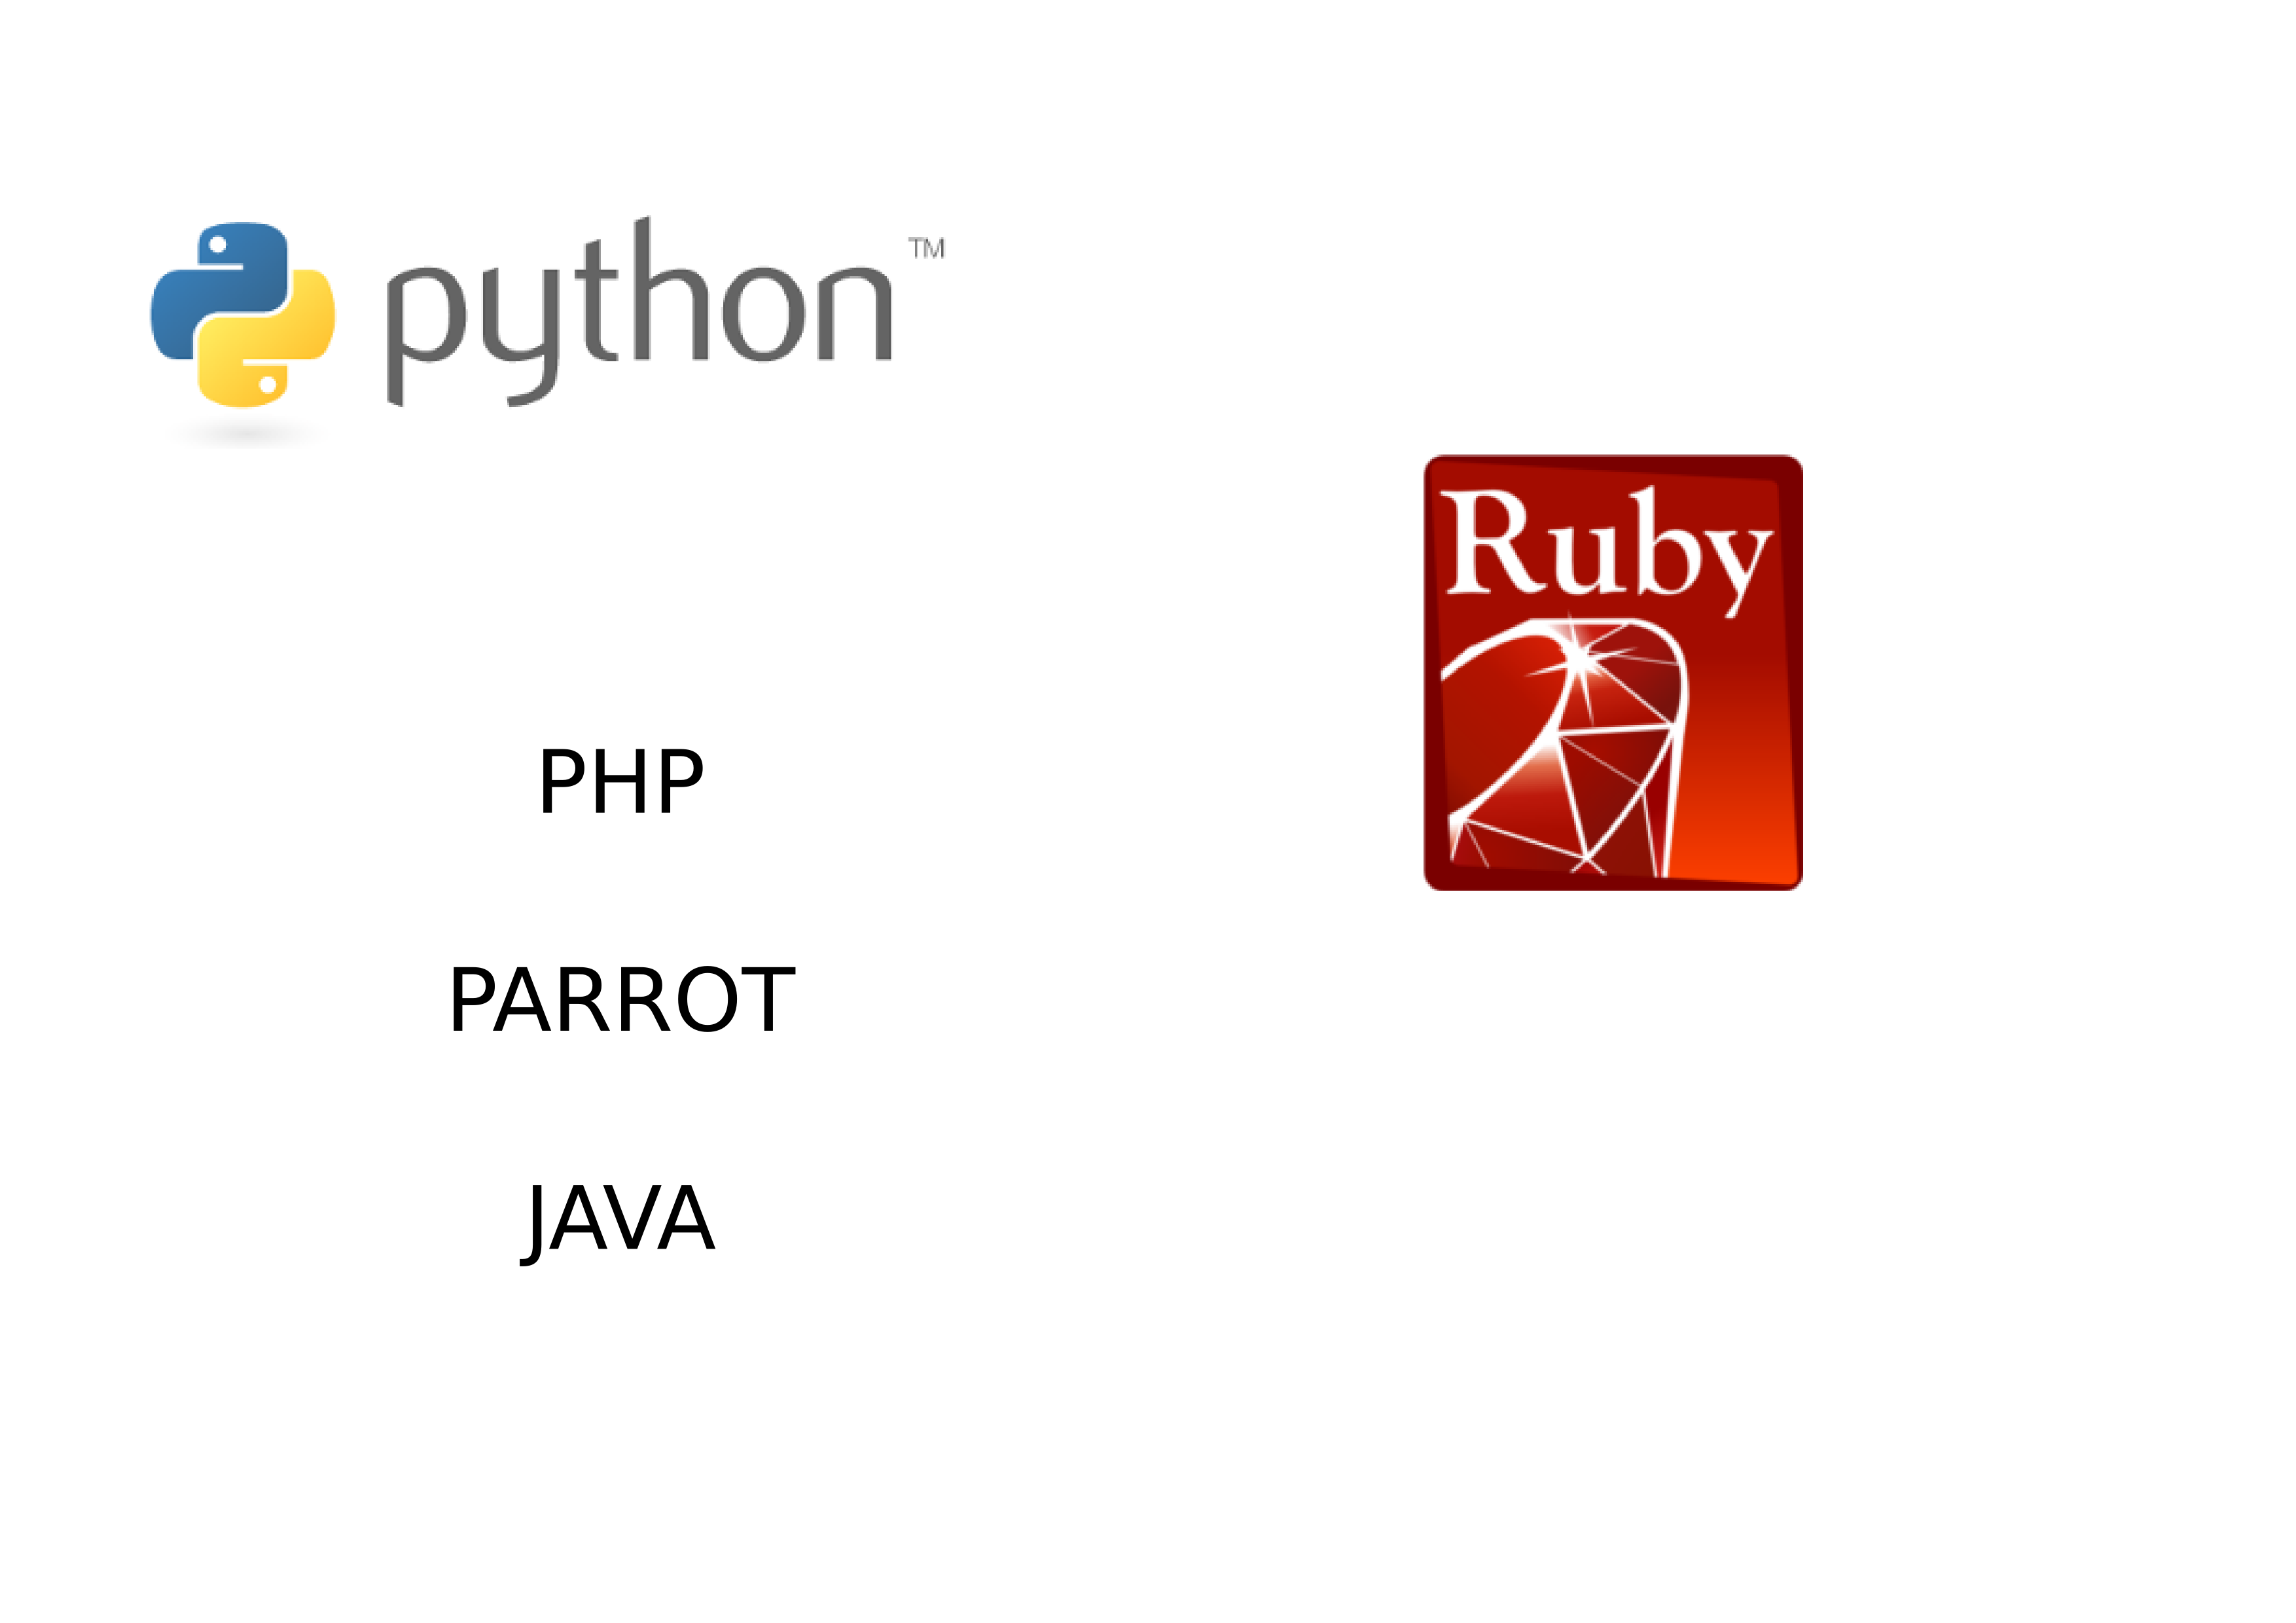
\includegraphics[scale=0.3]{img/sample-containers.png}
      \caption{Quelques conteneurs d'exécution les plus utilisés}
      \label{sample-containers}
    \end{center}
  \end{figure}
}

\ifslide{
  \begin{frame}{Quelques conteneurs d'exécution}
   \begin{center}
     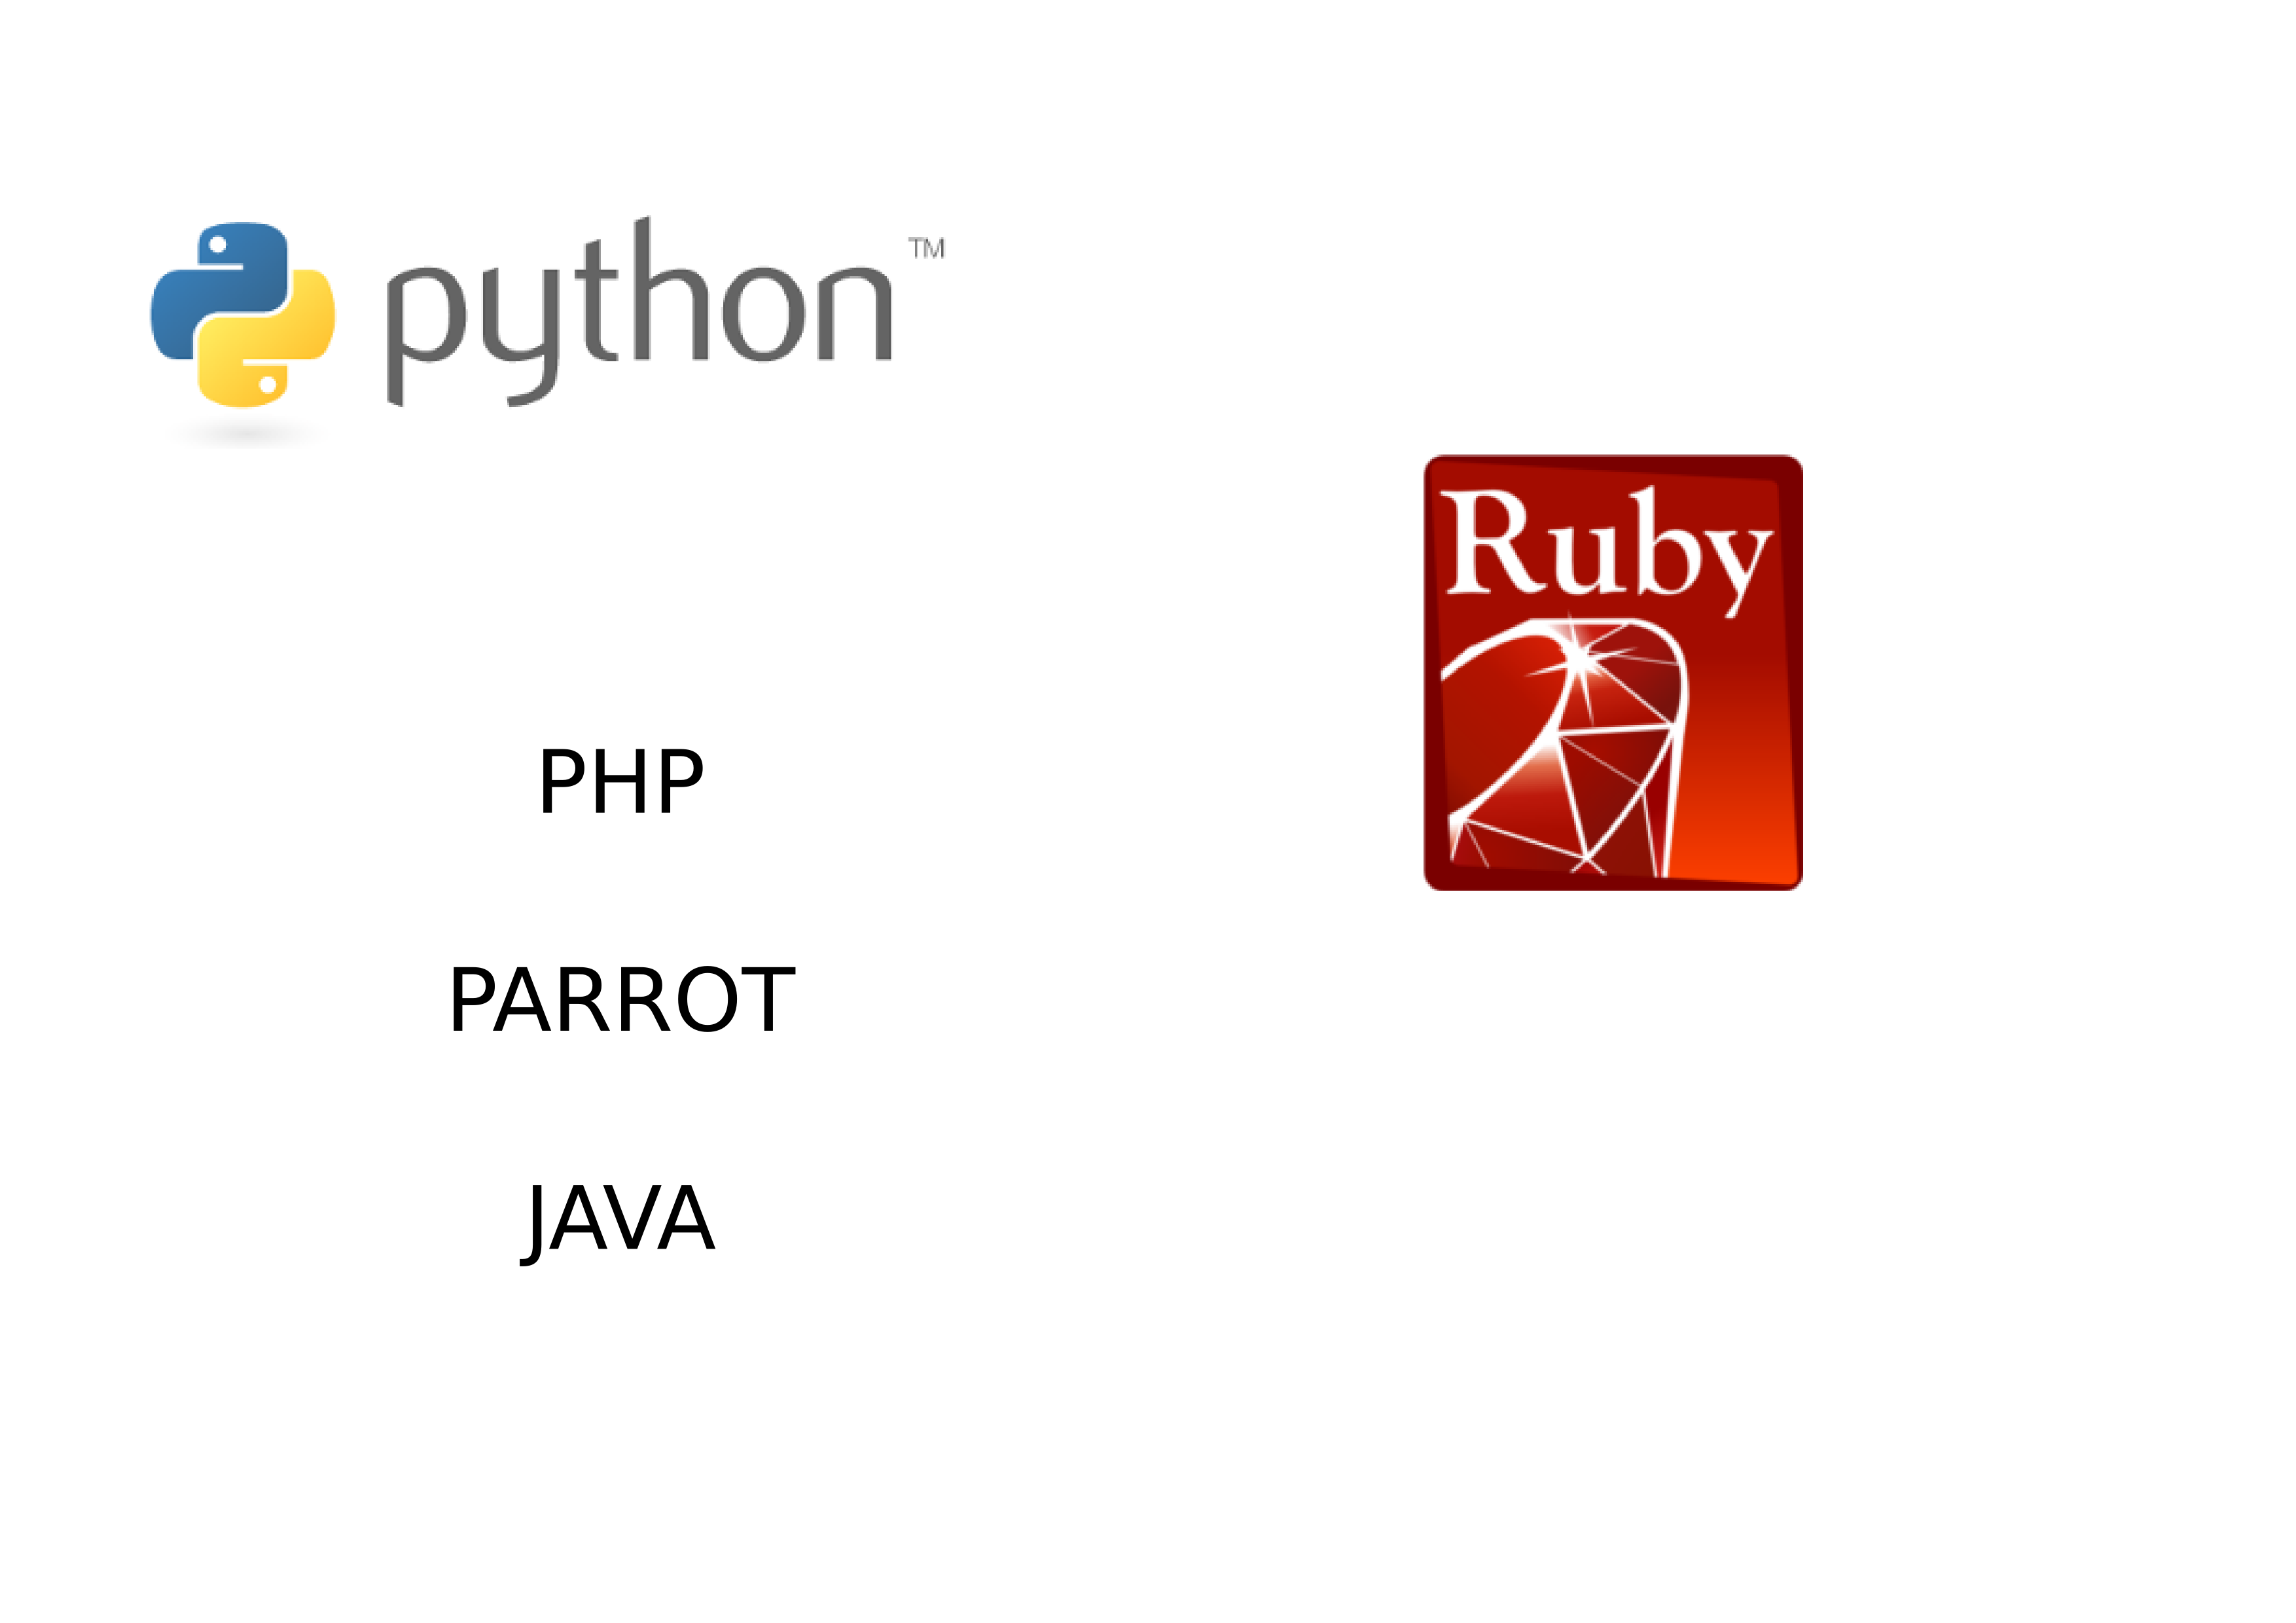
\includegraphics[scale=0.3]{img/sample-containers.png}
   \end{center}
  \end{frame}
}

\ifbook{
  \paragraph{} Si les conteneurs d'exécution abstrait le programme du système d'exploitation sur
  lequel il s'exécute, il est donc ainsi possible d'écrire un même programme Java ou un script
  Python de telle manière qu'il s'exécute de manière similaire sur différents système d'exploitation.

  \paragraph{} Il est donc ainsi possible d'écrire un même programme Java ou un script Python pour
  qu'il s'exécute de manière similaire sur différents systèmes d'exploitation. Attention néanmoins,
  il faut prendre soin de veiller à cette \textbf{interopérabilité} lors de la conception du
  programme, car l'on peut toujours aisément rendre son code très adhérant aux systèmes
  d'exploitation.

  \paragraph{} Attention néanmoins, si cette \textbf{interopérabilité} est rendue possible par
  l'utilisation d'un conteneur d'exécution, il faut néanmoins prendre soin de l'assurer lors de la
  conception du programme. En effet, on peut toujours aisément rendre son code très adhérant aux systèmes
  d'exploitation utilisés, et ceci malgré l'abstraction offerte par le conteneur.

  \paragraph{} Un exemple très concret de ce dernier point est l'utilisation de chemin de fichier
  spécifique à Windows©, plutôt que d'utiliser des URLs ou un chemin de fichier standard:

  \begin{figure}[hb]
    \begin{center}
      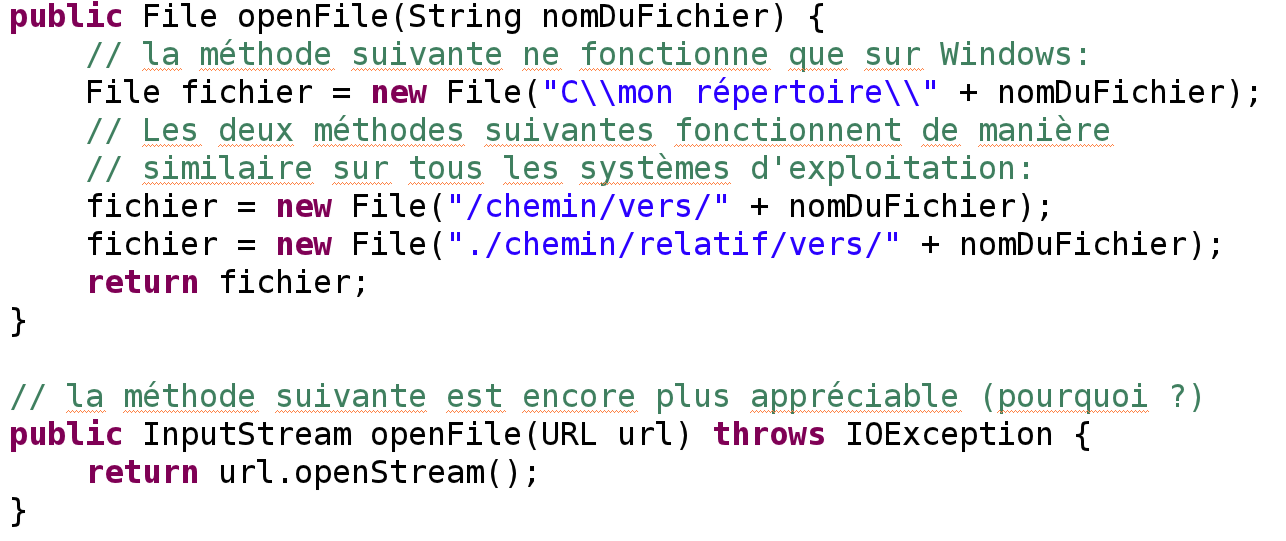
\includegraphics[scale=0.3]{img/interop.png}
      \caption{Exemple de problématique de portabilité au sein d'un conteneur}
      \label{interop}
    \end{center}
  \end{figure}
}

\ifslide{
  \begin{frame}{Interopérabilité}
   \begin{center}
     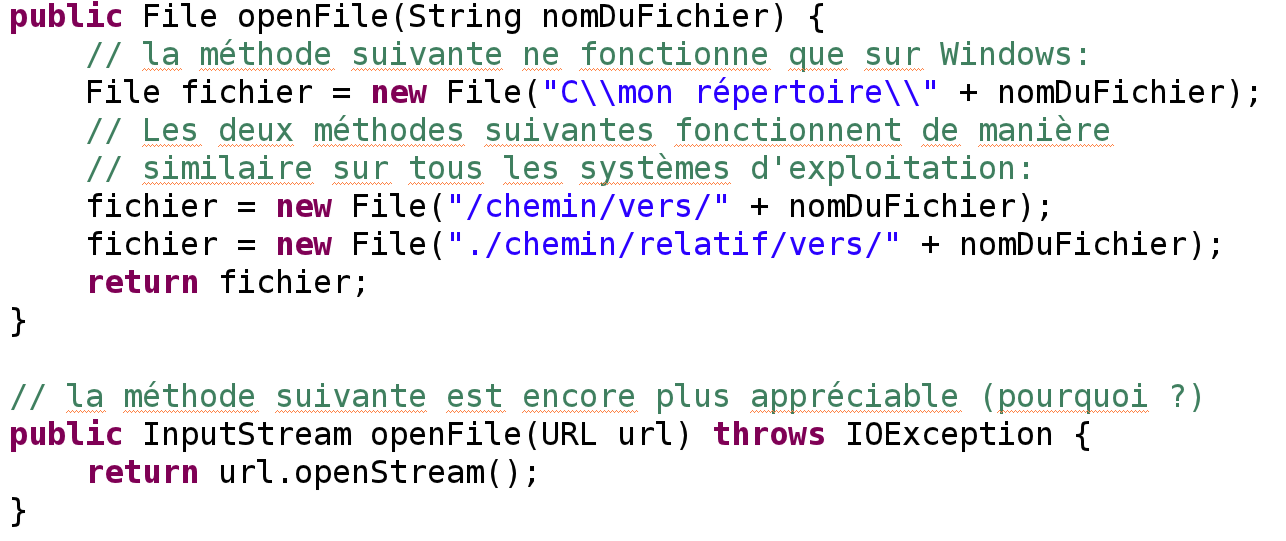
\includegraphics[scale=0.25]{img/interop.png}
   \end{center}
  \end{frame}
}

\ifbook{
  \paragraph{} C'est donc à propos des applications développées sur ces nouveaux conteneurs
  d'exécution, et non plus de manière \textbf{native}, que nous allons désormais discuter. On
  notera, au passage, que, au bout du compte, ces conteneurs d'exécutions forment un premier
  \textbf{Middleware} pour l'application.
}

\mysubsection{Serveur d'applications}

\ifbook{

  \paragraph{} À l'aide des conteneurs précédemment évoqués, nous avons maintenant un cadre robuste et
  portable d'exécution de programme, nous offrant déjà des primitives relatives élaborées. Néanmoins,
  ces contextes d'exécution sont toujours conçus pour exécuter un seul programme. Certes, ce programme
  peut créer des sous processus, mais en essence, le conteneur n'est pas conçu pour exécuter
  différentes applications de manière concurrente.

  \paragraph{} Nous allons voir apparaître la notion de \textbf{serveur d'applications} - avec un 's'
  à applications, car l'enjeu est bien ici de pouvoir exécuter et \textbf{administrer} plusieurs
  applications s'exécutant au sein d'un même et unique contexte d'exécution.

  \paragraph{} Voyons d'abord une définition du terme serveur d'applications pour éclaircir un peu le
  sujet. La définition suivante est issue de \mylink{http://TODO/}{Wikipédia} (accédé le 21/12/2011):

  \paragraph{} \textit{Un serveur d'applications est un logiciel d'infrastructure offrant un contexte
  d'exécution pour composants applicatifs. [...] Dans un sens strict les composants hébergés par le
  serveur d'applications ne sont pas de simples procédures ou scripts mais de réels composants
  logiciels conformes à un modèle de composants (EJB, COM, Fractal,...)}

  \paragraph{} Comme l'illustre assez bien la définition, ce serveur d'applications, qu'il s'agisse
  d'un serveur d'application Java/JEE ou d'un serveur python tel que WebWare, est au final un
  \textbf{produit d'intégration}. En effet, ce serveur a aussi pour rôle de faciliter, pour les
  applications qu'il héberge, l'utilisation de programmes connexes, tel que les bases de données ou un
  serveur d'authentification. Ainsi, le serveur d'applications permet l'intégration des applications à
  d'autres applications qui lui seront nécessaires.

  \paragraph{} Comme l'indique la définition, il est important de noter aussi qu'un serveur
  d'application abrite des \textbf{composants applicatifs}, et non de simple API. Le comportement de
  ces composants est ainsi beaucoup plus configurable et ils offrent, pour la plupart, et à l'inverse
  des API, des mécanismes d'administration. En outre, les composants, là encore à l'inverse des APIs,
  sont plus "actifs". Nous reviendrons sur ce point tout au long du cours.

}

\ifbook {
  %TODO: definition d'un pool de connexion, intérêt...
  \mysubsubsection{Pool(s) de connexion}

  \paragraph{} Plutôt que de continuer de faire un résumé très théorique, et vraisemblablement peu
  pertinent sur ce sujet - qui ne ferait que satisfaire un goût très Mésopotamien de l'inventaire et
  des catalogues, nous allons voir un petit cas pratiques de configuration d'un pool de connexion.

  \paragraph{} Cette démarche sera, espérons le, un peu moins aride, et devrait surtout permettre au
  lecteur de bien saisir les concepts sous jacents. Pour être didactique, cette section contiendra
  donc des extraits de codes et de configuration, mais là encore, l'objectif pédagogique ne sera pas
  de retenir, ni même de forcément comprend l'intégralité de ces extraits, mais de bien cerner, de
  manière concrète, les concepts de plus haut niveau qui s'y rapportent.

  % TODO: RMI appli avec une connecion, qui dure 60s, renvoie une * toutes les 5s - barre de
  % progression - timeout, puis 2 utilisateurs concurrent
  % HTTP, RMI, AJP => offre pool de connexion, partagé entre les applications

  \mysubsubsection{Threads}
}

%\ifslide{
%  \demoframe{Threads}{
%    \begin{block}{Configuration d'un "pool" de connexion}
%      \begin{itemize}
%        \item
%      \end{itemize}
%    \end{block}
%  }
%}

\ifbook{

  \paragraph{} De la même manière dont il existe un \textit{pool} de connexion, dont la gestion est
  confiée au serveur d'applications, la gestion du nombre de sous processus, ou plutôt de
  \textit{thread} pour reprendre le terme anglais plus souvent utilisé, est, elle aussi, confiée au
  serveur d'application.

  \paragraph{} Dans une suite logique à ce que nous venons de voir, nous allons voir comment
  augmenter ou réduire le nombre de \textit{threads} qu'une application, s'exécutant au sein de
  JBoss, peut utiliser.

  \mysubsubsection{Première conclusion}

  \paragraph{} En étudiant, de manière sommaire, la gestion de types distincts de ressources (d'une
  part des connexions à une source de données, d'autres part le nombre de thread), nous pouvons
  désormais un peu mieux comprendre le rôle du serveur d'applications.

  \paragraph{} Réel produit d'intégration, le serveur d'applications prend donc en charge la gestion
  de nombreux, si ce n'est tous, aspects techniques, laissant les applications utilisées de simple
  API, standard pour la plupart. Une fois déployé au sein du serveur, on dispose néanmoins de
  nombreux mécanismes pour régler et configurer l'utilisation des ressources par l'application, de
  manière à exploiter au mieux possible ces dernières.

  \begin{figure}[hb]
    \begin{center}
      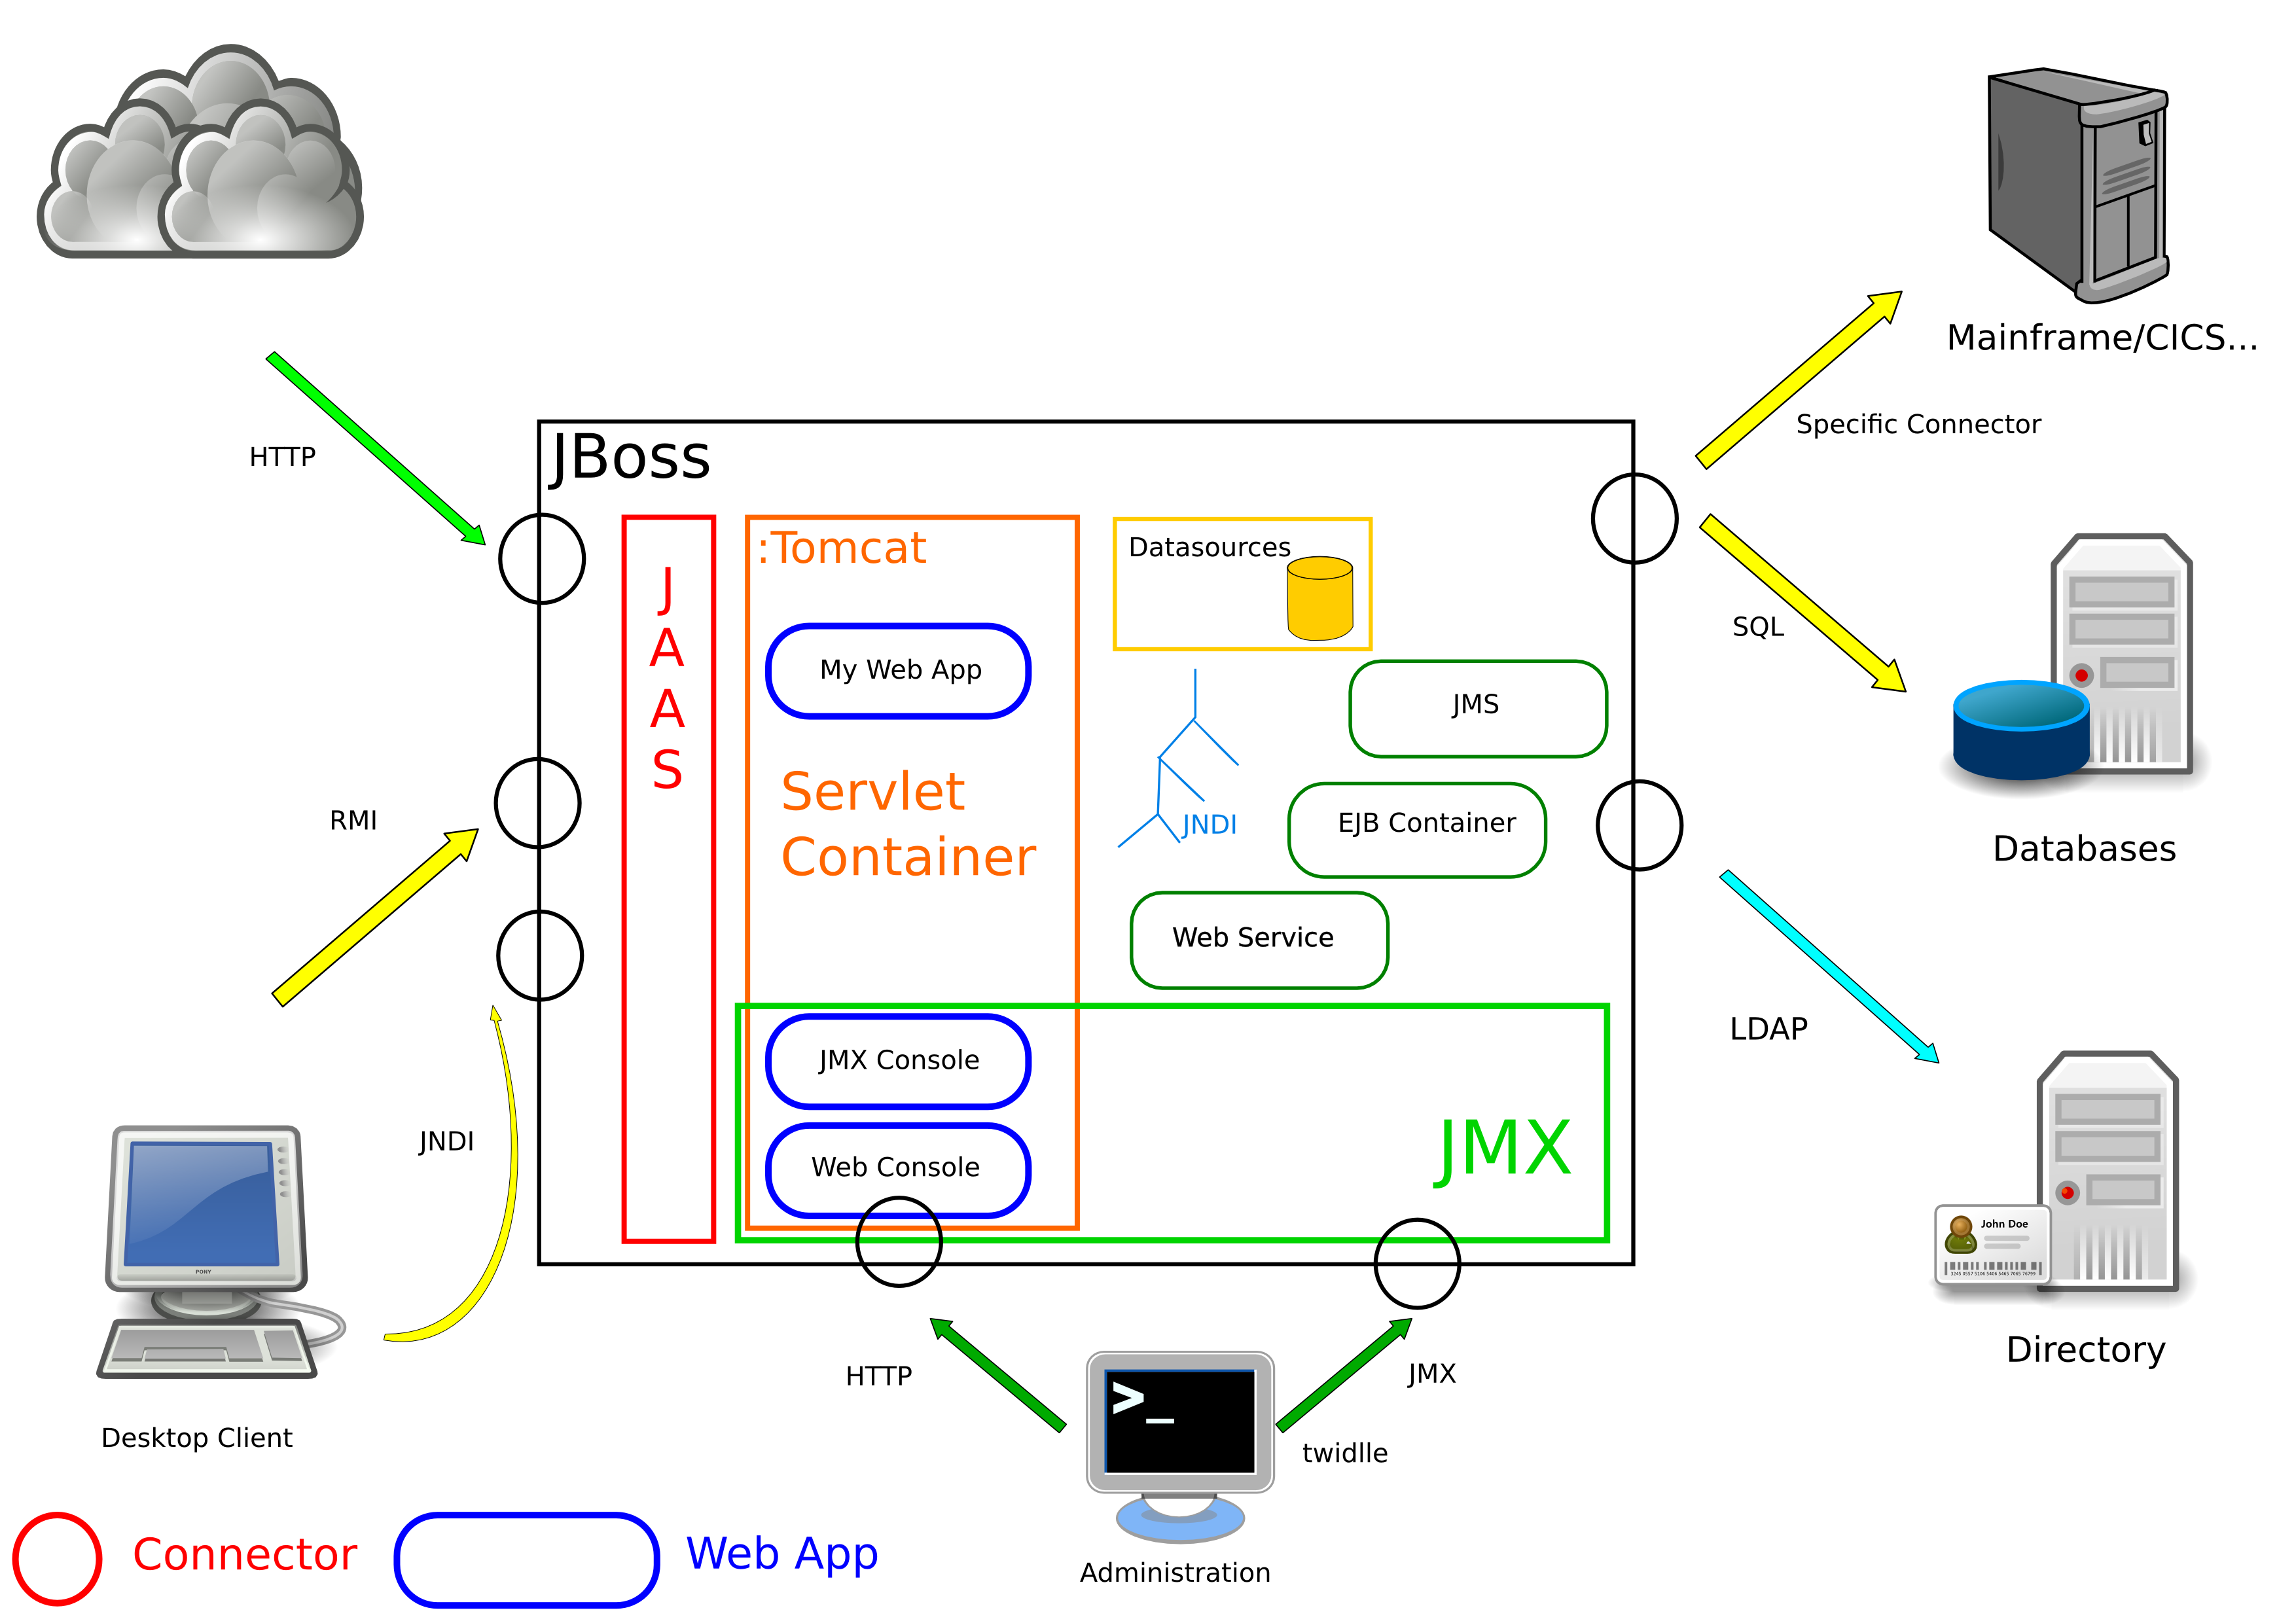
\includegraphics[scale=0.4]{img/integration-product.png}
      \caption{Exemple de serveur d'application: JBoss}
      \label{integration-product}
    \end{center}
  \end{figure}
}

\ifslide{
  \begin{frame}{Vision d'ensemble d'un serveur applicatif (JBoss AS)}
   \begin{center}
     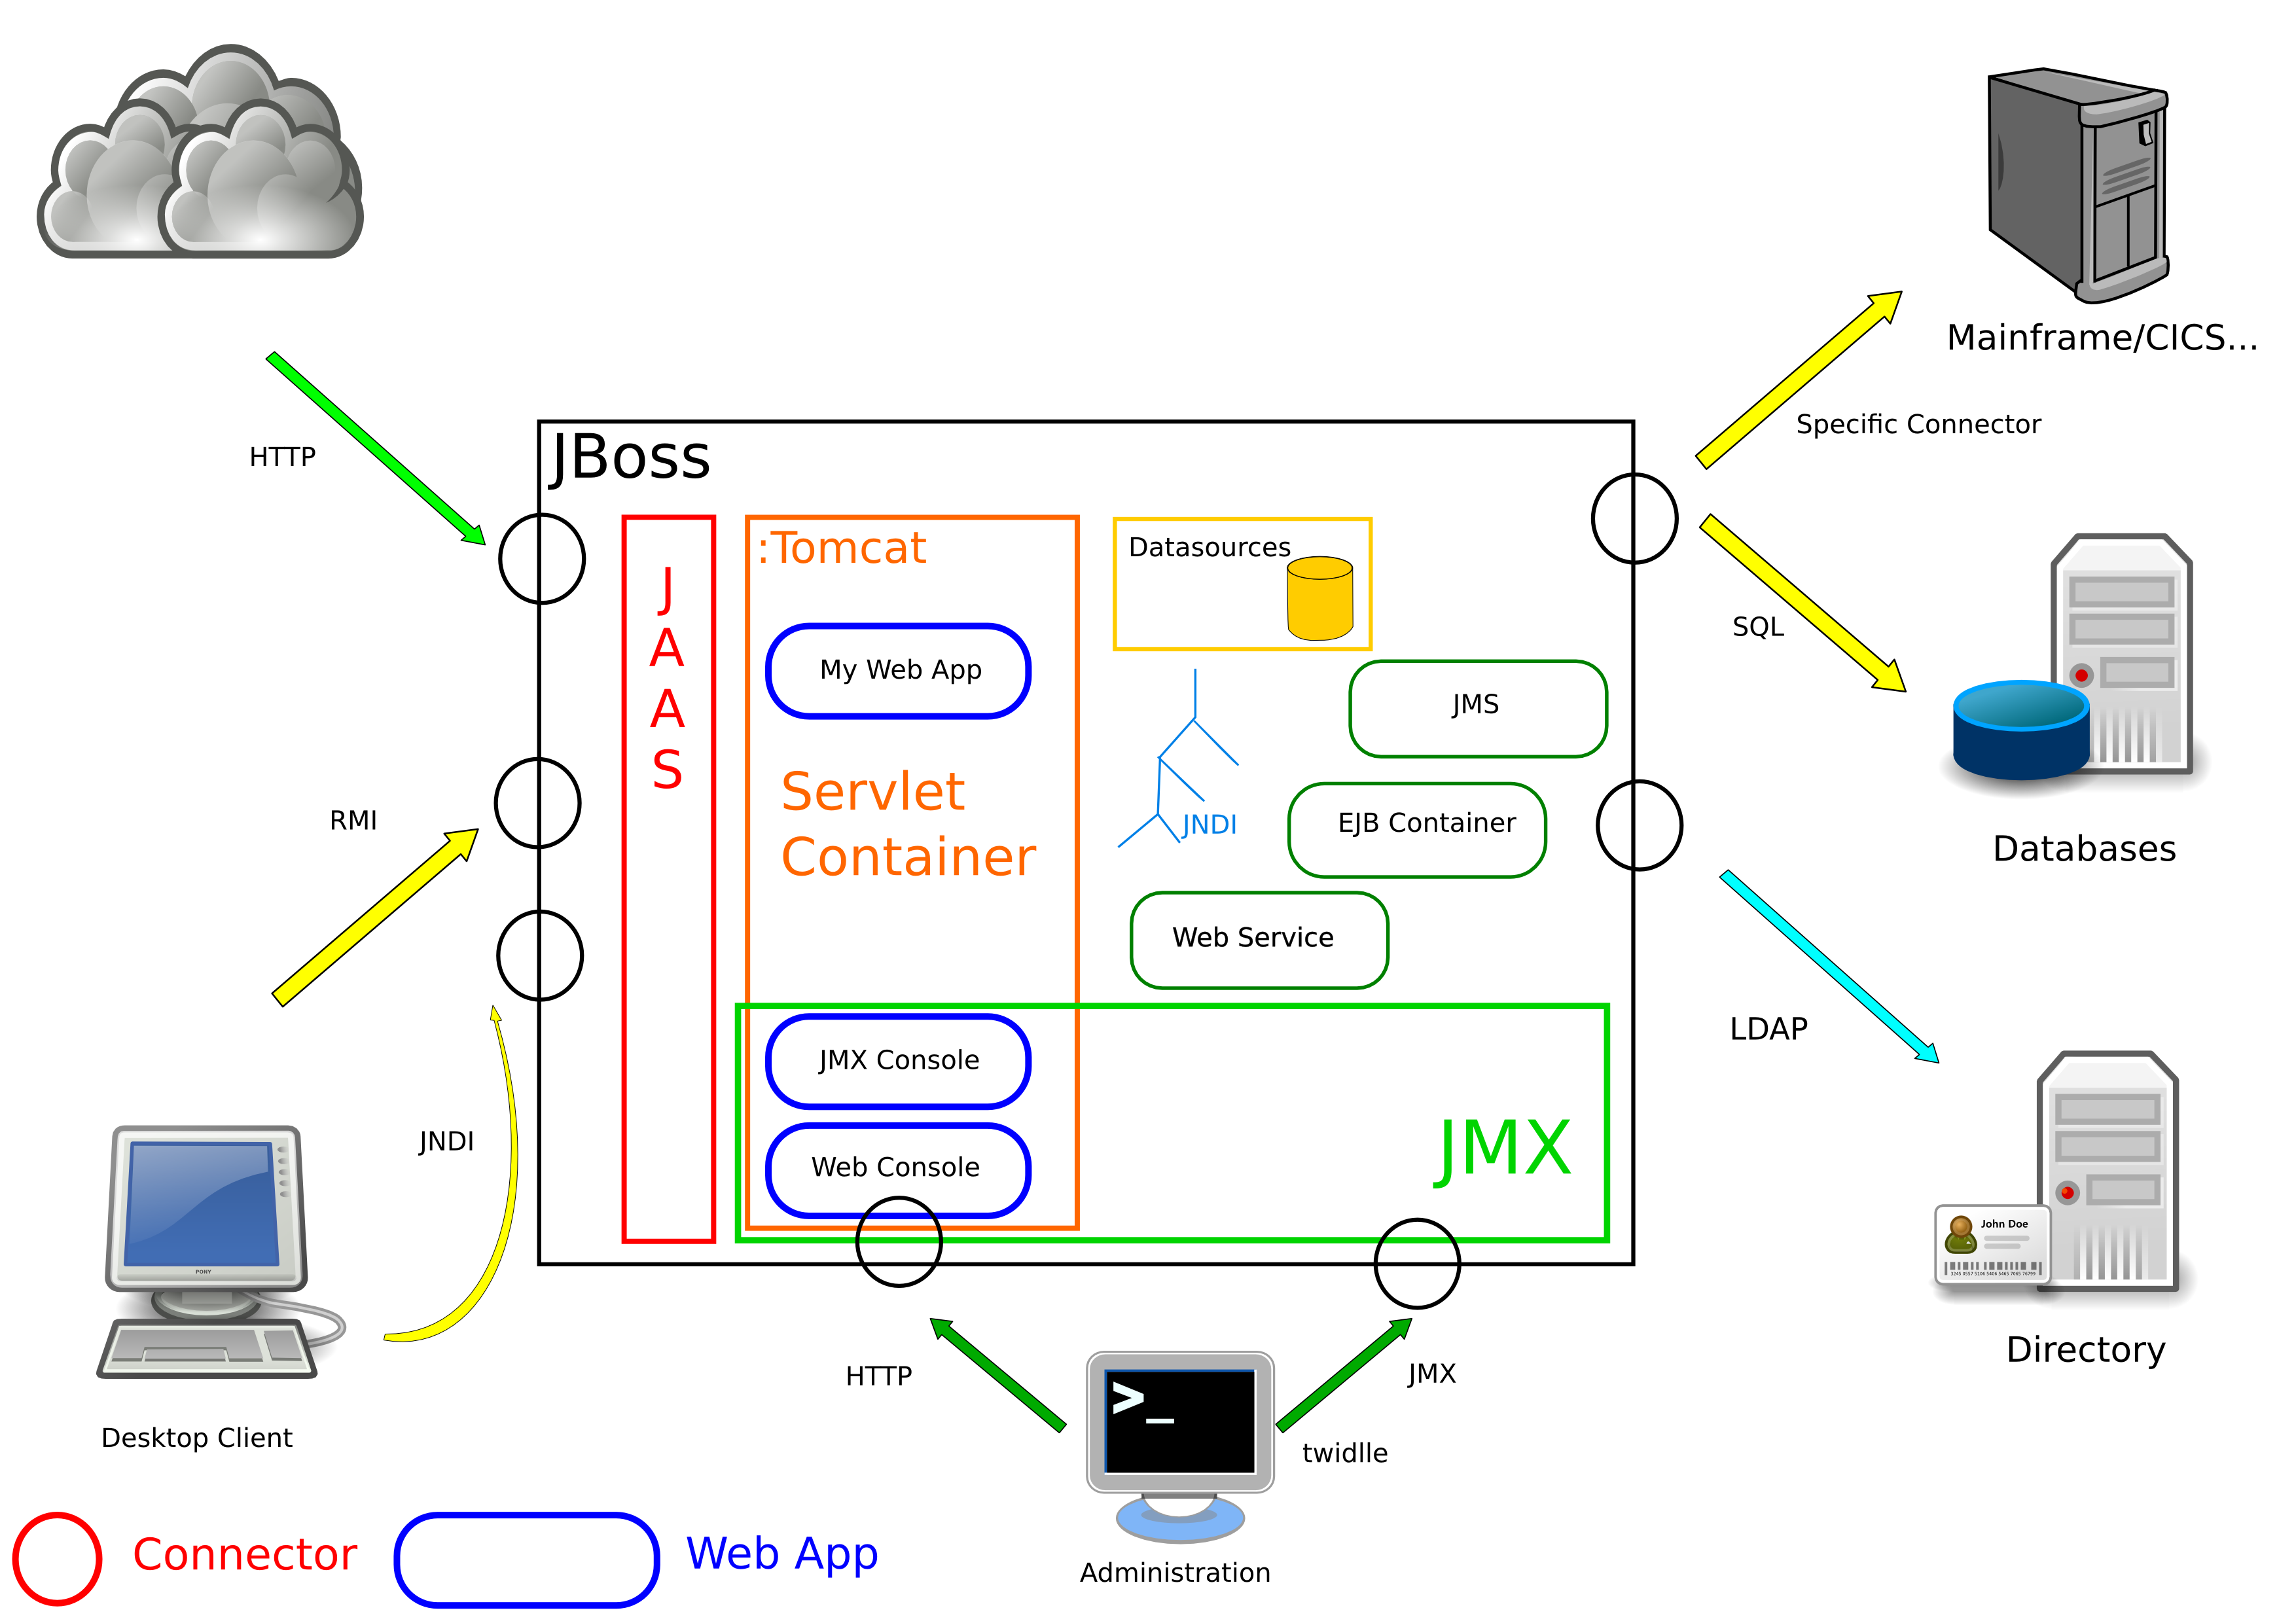
\includegraphics[scale=0.3]{img/integration-product.png}
   \end{center}
  \end{frame}
}

\newpage
\mysubsection{Conteneur "Web"}

\ifbook{

  \paragraph{} Comme nous venons de le voir, un serveur d'applications héberge donc des
  \textbf{applications}, et leur offre, via des \textbf{API}, idéalement standards, l'accès à de
  nombreux \textbf{services}, déployé en son sein, sous forme de \textbf{composants}. Bien qu'il
  soit tout à fait possible de réaliser une application de type client/serveur
  "traditionnel"\footnote{Par "traditionnel", on entend ici une application n'utilisant pas les
  technologies spécifique au "Web"}, la plupart des applications déployées dans un serveur
  d'applications sont des applications "web". Ainsi, l'un des \textbf{composants} clés du serveur
  est son \textbf{conteneur web}.

  \paragraph{} Cette section s'intéresse donc tout particulièrement au services fournies par ce
  composant aux applicatifs exécutées par le serveur d'applications. Encore une fois, il est
  possible que certains des détails techniques évoqués dans cette partie soient plus ou moins
  spécifique au conteneur de servlet (TODO) du monde Java ou même à des produits spécifiques, tel
  Tomcat ou JBoss Web, mais, dans l'ensemble, quelques soit sa technologie, un serveur d'application
  devrait proposés la plupart de ces fonctionnalités aux applications qu'il déploie.

  \mysubsubsection{Support du protocole HTTP}

  \paragraph{} Comme décrit dans une précédente partie, HTTP est un protocole texte ouvert et
  standardisé. Bien qu'il soit possible pour un programmeur d'implémenter lui même un serveur
  supportant ce protocole, il est évidemment beaucoup plus pertinent de disposer d'une API,
  spécifique au langage utilisé, fournissant directement, sous forme de primitives manipulables
  aisément toutes les informations associées fournies par ce protocole dans le cadre d'un échange
  entre un client HTTP, un navigateur "web", et une application "web".

  \paragraph{} Illustrons ce point par l'exemple, en étudiant l'API Java des Servlets. Cette API a
  été conçue pour faciliter le plus possible le développement d'application "web". Elle permet, en
  effet, de simplement étendre une classe existente pour créer un nouveau programme ou disons plutôt
}

\ifslide{
 \demoframe{Un rapide tour de l'API Servlet}{
   % FIXME: add a nice picture for servlet API tour
   \begin{block}{Squelette d'une application Web Java}
     \begin{itemize}
       \item le descripteur (\textit{web.xml})
       \item la servlet et son API
       \item ...
     \end{itemize}
   \end{block}
 }
}

\ifbook{
 \mysubsubsection{Session, gestion des entrées/sorties et exécution concurrente}
 \mysubsubsubsection{Java Servlet}
 \paragraph{} Le modèle proposée par les Servlet Java est assez élégant. En effet, il abstrait le
 programmeur de la complexité du protocle HTTP, fourni des objets Java simple à utiliser et fournit,
 au final, un cavenas, très similaire à celui d'un simple programme, pour développer son programme.

 \paragraph{} Au delà du support du protocole de HTTP, et du travail de \textit{marshalling}
 effectué par la Servlet pour le développeur, l'API Servlet apporte aussi un ensemble de fonctions
 simpe pour manipuler la Session.

 \paragraph{} Enfin, On notera au passage que le modèle abstrait intégralement le programmeur de la
 nature \textbf{concurrente} des applications Web. Le serveur exécutant cette Servlet se chargera de
 créer une instance de cette dernière par requête, et isolera ces exécutions les uns des autres.

 \paragraph{} Maintenant, il est évident que construire intégralement une page Web, de manière
 programmatique, à travers les primitives offertes par l'API Servelt, est une tâche très laborieuse
 et redondante. En outre, adopter cette stratégie à aussi pour désagréable effet de bord,
 d'allégrement mélanger le code \textbf{métier} - les traitements effectués sur les données
 manipulées par l'applicatif, et les informations associées à la \textbf{présentation} (structure de
 la page HTML) de ces dernières.

 \mysubsubsubsection{JSP}
 \paragraph{} Pour faciliter la conception rapide de page web et, surtout séparer la présentation
 des données de leurs traitements, la spécification associée aux Servlets a été enrichi pour offrir
 une syntaxe plus approprié, désigné sous le nom de Java Server Pages, ou JSP.

 \paragraph{} Plutôt que de construire intégralement une page HTML au sein d'un code Java, les JSPs
 inverse le paradigme, permettant simplement d'écrire une page HTML habituelle, injectant le code
 \textbf{métier} dans les seuls parties où il est requis.

 \paragraph{} Ainsi, une page JSP peut aisément être manipulée, et surtout modifier, par un
 ergonome ou un graphiste, sans pour autant nécessiter de modifier le code métier.

 \paragraph{Remarque} Si JSP est clairement spécifique à Java, l'approche ne l'est en aucun cas. Le
 succès de PHP s'explique beaucoup par le fait qu'il propose la même approche, et, dans le monde
 Microsoft, le langage ASP suit le même concept.

}

\newpage
\mysubsection{Transaction}

\ifbook{

  \paragraph{} La plupart des applications en ligne ont généralement comme objectif de réaliser des
  \textbf{transactions}. On mesure d'ailleurs très souvent la performance d'un système au nombre de
  transactions effectuées par minute. La notion de transaction est donc au coeur de bien des aspects
  du \textbf{middleware}.

  \paragraph{} Bien que l'usage du terme \textbf{transaction} soit très répandu, son sens n'est
  forcément aussi clairement maîtrisé. En outre, chaque application a, dans les faits, sa propre
  définition et compréhension de la notion de transaction.

  \paragraph{} Nous allons donc commencer par étudier sa définition plus ou moins académique. D'après
  \mylink{http://fr.wikipedia.org/wiki/Transaction\_informatique}{Wikipédia} la définition d'une
  transaction (accédée le 27/12/2011) est la suivante:

  \paragraph{} \textit{En informatique, et particulièrement dans les bases de données, une
  transaction telle qu'une réservation, un achat ou un paiement est mise en oeuvre via une suite
  d'opérations qui font passer la base de données d'un état A - antérieur à la transaction - à un
  état B postérieur et des mécanismes permettent d'obtenir que cette suite soit à la fois atomique,
  cohérente, isolée et durable (ACID):}

  \begin{description}
    \item[atomique] \textit{la suite d'opérations est indivisible, en cas d'échec en cours d'une des
    opérations, la suite d'opérations doit être complètement annulée (rollback) quel que soit le
    nombre d'opérations déjà réussies.}
    \item[cohérente] \textit{le contenu de la base de données à la fin de la transaction doit être
    cohérent sans pour autant que chaque opération durant la transaction donne un contenu cohérent.
    Un contenu final incohérent doit entraîner l'échec et l'annulation de toutes opérations de la
    transaction.}
    \item[isolée] \textit{lorsque deux transactions A et B sont exécutées en même temps, les
    modifications effectuées par A ne sont ni visibles par B, ni modifiables par B tant que la
    transaction A n'est pas terminée et validée (commit).}
    \item[durable] \textit{Une fois validé, l'état de la base de données doit être permanent, et
    aucun incident technique (exemple: crash) ne doit pouvoir engendrer une annulation des
    opérations effectuées durant la transaction.}
  \end{description}

  \begin{figure}[hb]
    \begin{center}
      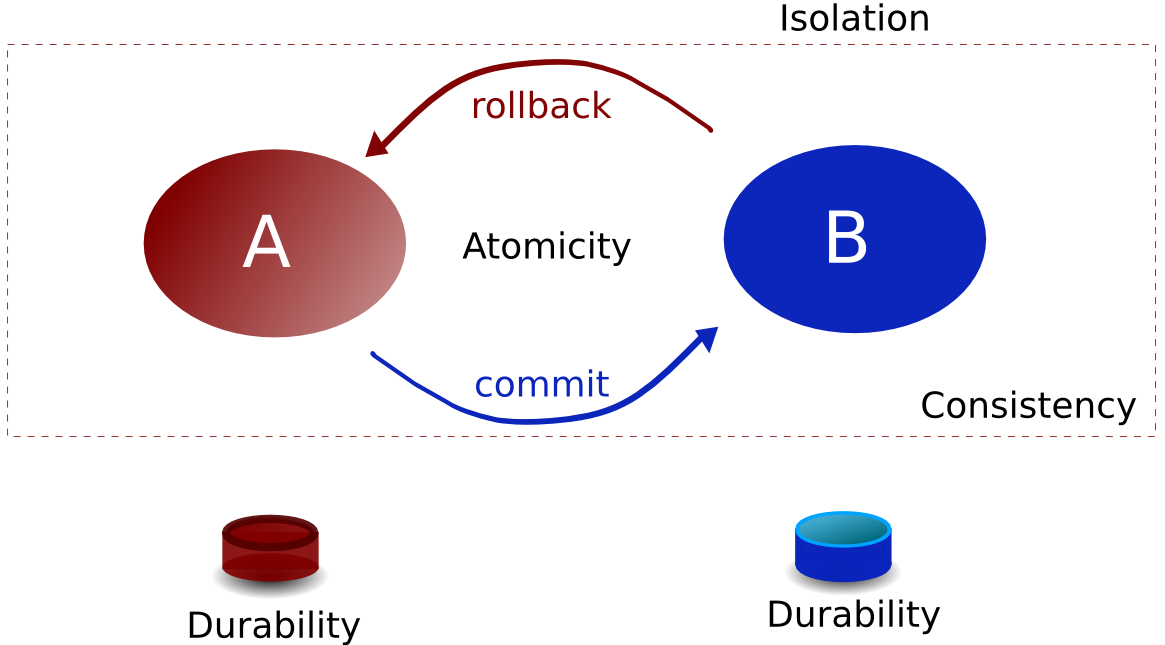
\includegraphics[scale=0.25]{img/transaction.png}
      \caption{Caractéristique d'une transaction}
      \label{tx}
    \end{center}
  \end{figure}
}

\ifslide{
  \begin{frame}{Transaction}
   \begin{center}
     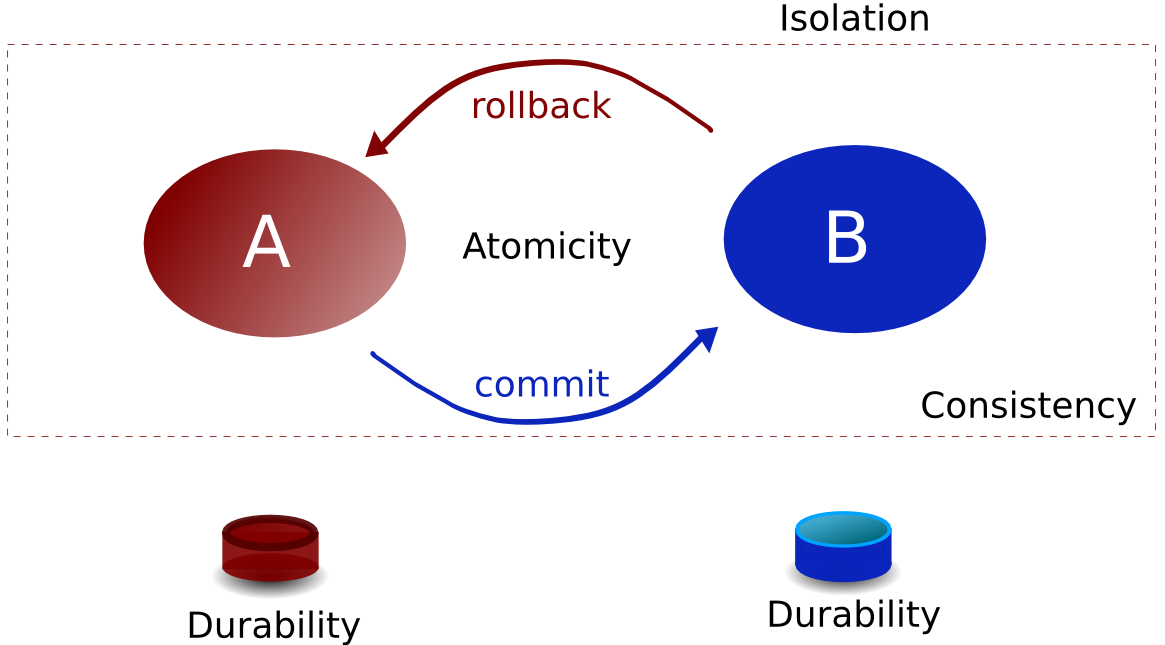
\includegraphics[scale=0.3]{img/transaction.png}
   \end{center}
  \end{frame}
}

\ifbook{

  \mysubsubsection{Atomicité des transactions}

  \paragraph{} L'aspect transactionnel de la plupart des opérations effectuées par un système
  informatique est un point important car c'est souvent à la charge du serveur d'applications ou du
  \textit{middleware} utilisé par l'application de l'assurer.

  \paragraph{} La caractéristique principale d'une transaction est son \textbf{atomicité}. En effet,
  à la fin de l'exécution d'une opération transactionnelle, on se retrouve soit dans un nouvel état
  (un \textbf{commit} a été effectué) ou dans l'état initial (un \textbf{rollback} a été réalisé).
  En outre, une transaction est très souvent une unité insécable, elle ne peut être découpée en
  plusieurs sous opérations distinctes, elle doit se réalise (ou non) au sein d'une opération, qui
  est donc atomique.
}

%% TODO: slide on tx isolation
\ifbook {

  \mysubsubsection{Isolation des transactions}

  \paragraph{} Les transactions s'exécutent la plupart du temps en parallèle les unes ou autres, il
  est donc crucial de correctement orchestrer ces opérations concurrentes pour s'assurer d'un
  résultat concurrent. C'est l'isolation d'une transaction qui garantit ce état cohérent.

  \paragraph{} L'isolation a pour conséquent concrète d'empêcher deux transactions de modifier de
  manière concurrente un objet. Si deux transactions concurrentes souhaitent modifier le même objet,
  l'une prendra la priorité et la seconde attendra la fin de cette dernière.

  \paragraph{} Un autre enjeu de l'isolation d'une transaction est de masqué les éventuels états
  intermédiaires obtenues lors de son exécution. À l'insu de la transaction, on se trouve dans
  l'état souhaité ou dans l'état initial, mais en aucun cas, dans un état intermédiaire.

  \paragraph{} Néanmoins, sérialiser systématiquement les transactions pose de gros problèmes de
  performances, et ce n'est donc pas toujours possibles. Certains systèmes, tel que la plupart des
  bases de données, utilise donc un système de contrôle actifs des opérations concurrentes, et
  n'isole donc pas leurs transactions.

  \paragraph{} On peut donc déjà noter qu'une transaction n'a que deux statuts de fin d'exécution
  possible:

  \begin{itemize}
    \item \textbf{commit}
    \item \textbf{rollback}
  \end{itemize}

  \begin{figure}[hb]
    \begin{center}
      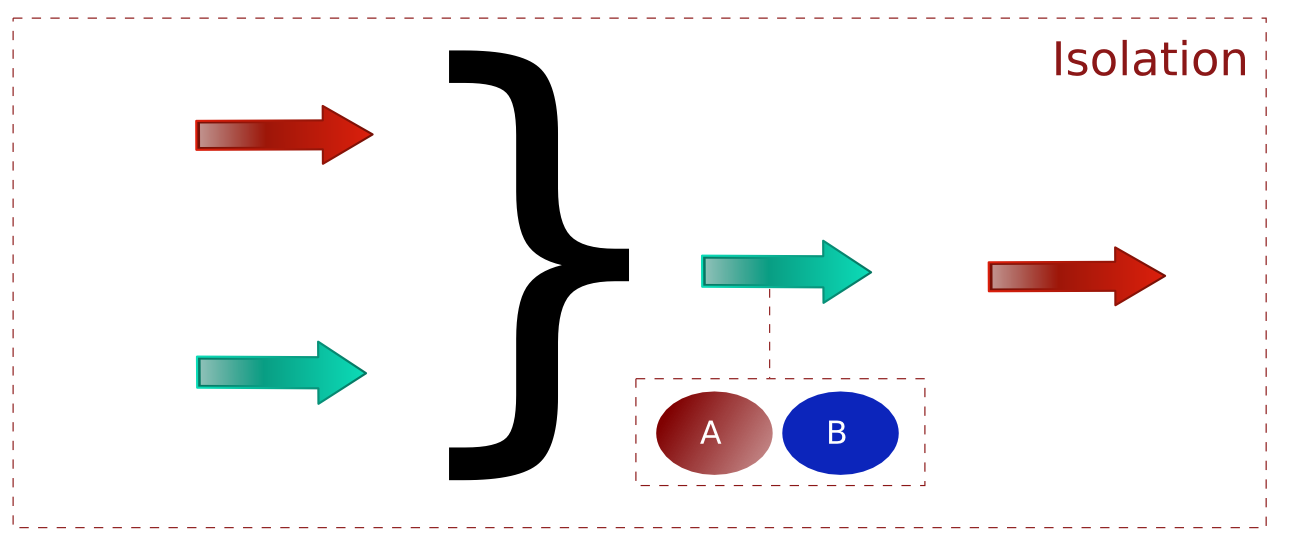
\includegraphics[scale=0.3]{img/tx-isolation.png}
      \caption{Isolation d'une transaction}
      \label{tx-isolation}
    \end{center}
  \end{figure}
}

\ifslide{
  \begin{frame}{Coût en performance d'une transaction}
   \begin{center}
     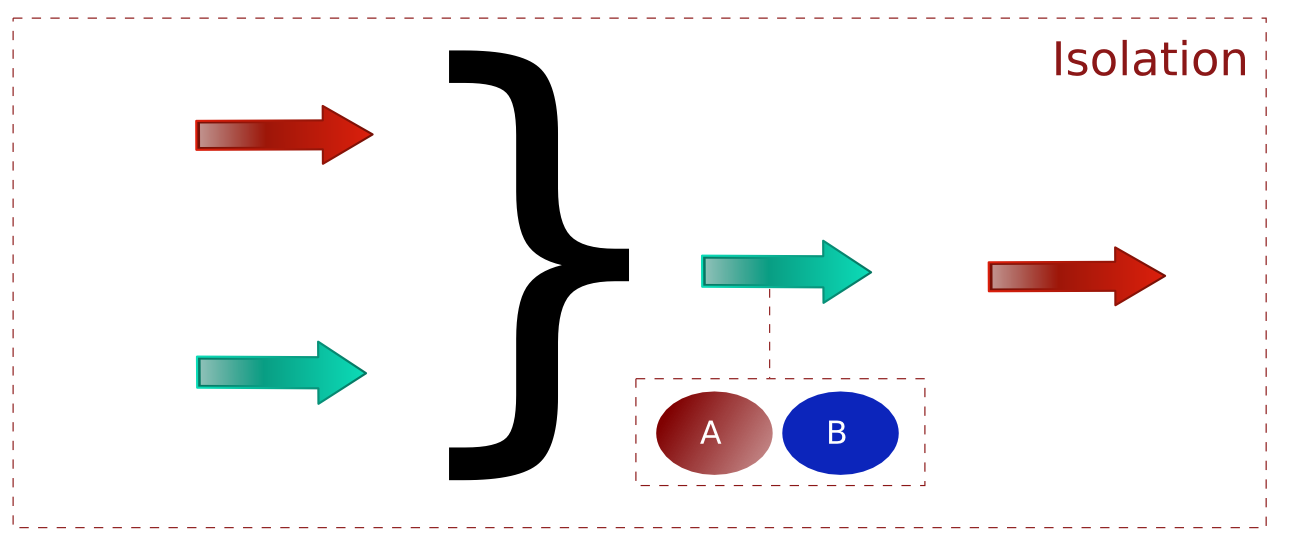
\includegraphics[scale=0.25]{img/tx-isolation.png}
   \end{center}
  \end{frame}
}

\ifbook {
  \mysubsubsection{Sémantique d'une transaction}

  \paragraph{} La théorie derrière la notion de transaction dispose, comme toute théorie, de sa
  propre sémantique, offrant un certain niveau d'abstraction. Pour décrire la réalisation d'une
  transaction, on désigne les différents systèmes entre en jeu sous les noms suivants:

  \begin{itemize}
    \item les \textbf{participants} sont les différents systèmes impliqués dans la transaction ;
    \item \textbf{coordinateur} est le système qui se charge de coordonner les participants.
  \end{itemize}

  \paragraph{} Plus concrètement, au début d'une transaction, le \textbf{coordinateur} demande à
  chaque \textbf{participants} si ils sont près à effectuer leur \textbf{commit}. Une fois que tous
  ont répondu de manière favorable, le coordinateur demande à tous d'effectuer l'opération, et
  retourne et l'état de \textbf{commit} est retourné.

  \paragraph{} Dans la théorie, bien évidemment, les participants sont garant de leur état, et, si
  ils s'engagent à pouvoir effectue leur \textbf{commit}, ils ne peuvent en aucun cas échoué par la
  suite. Dans la pratique, il est difficile de garantir une telle robustesse\footnote{Spécialement,
  pour garantir que leur opération soit ACID, les systèmes doivent pouvoir obtenir un
  \textbf{verrou} sur la ressource qu'il manipule, et, dans la pratique, c'est en fait très
  difficile à mettre en place...}.

  \paragraph{} Ce mécanisme de transaction est souvent désigné sous le nom de \textbf{two phase
  commit}. En effet, ce dernier se déroule en deux phases, une de préparation où chaque participants
  s'engagent (ou non) à effectuer un \textbf{commit}, et une seconde, où leur coordinateur déclenche
  l'exécution de ces opérations.

  \paragraph{} On notera que le protocole du \textbf{two phase commit} est très abstrait et ne
  préjuge en aucun cas d'une architecture logicielle ou physique. Le coordinateur, par exemple, peut
  s'exécuter au sein d'un même processus que la transaction ou être exécuté sur une autre physique.
}


%%TODO: slide on READ/WRITE, OPTIMIST/PESSIMIST

\ifbook{
  \subsubsection{Contrôle de la concurrence dans le "two phase commit"}

  \paragraph{} On peut simplifier les transactions exécutées par un système en deux catégorie : les
  transactions effectuant des opérations de lecture (\textbf{READ}) et celle d'écriture
  (\textbf{WRITE}). Il est évident que des opérations de lectures peuvent s'exécuter de manière
  concurrente sans nécessiter de verrou sur les données qu'elles accèdent.

  \paragraph{} À l'inverse, les opérations d'écriture nécessitent la mise en place d'un
  \textbf{verrou exclusif}. Ce dernier a pour rôle de bloquer d'éventuels autres opérations
  d'écriture que les opérations de lecture. En effet, ces dernières doivent accéder à un état cohérent, et
  non à un état intermédiaire, produit par l'opération d'écriture en cours d'exécution.

  \paragraph{} Pour optimiser ce fonctionnement, il existe deux \textbf{stratégies de
  verrouillage}\footnote{Il existe fait plus de stratégie, qui sont généralement des variations
  des deux présentés ici}:

  \begin{description}
    \item[Pessimiste] Cette stratégie part du principe que les opérations d'écritures concurrentes
    sont fréquentes, et opte donc pour utiliser systématiquement un verrou. En plus d'avoir un effet
    négatif sur les performances, cette stratégie augmente le risque d'apparition \textbf{deadlock} (que
    nous verrons plus loin), mais elle assure une forte cohérence des données obtenues.
    \item[Optimiste] Cette stratégie se fonde elle sur justement très peu d'opérations en écritures
    concurrentes et un très grand nombre d'opération en lecture. Pour assurer que ces derniers ne
    soient pas entraver par les opérations en écritures, ces dernières ne posent pas de verrou, et
    le système se contente d'effectuer un \textbf{rollback} en cas d'opération d'écriture
    concurrente.
  \end{description}
}

%% TODO: Slide on deadlock

\ifbook{

  \mysubsubsection{Deadlock}

  \paragraph{} Le principal intérêt des transactions réside dans la garantie sur la cohérence des
  données. En effet, l'utilisation de transactions assurent que si deux processus accèdent et
  modifient, de manière concurrente, la même donnée, l'une des opérations n'écrasera pas simplement
  le résultat de l'autre.

  \paragraph{} À ce regard, la transaction remplit un peu prêt le même rôle que le système
  d'exploitation dans l'arbitrage des accès aux données entre processus. Prenons un exemple
  simpliste, pour l'illustrer.

  \paragraph{} Si deux processus cherche à incrémenter une valeur A de manière concurrente,
  hors de toute transaction, le résultat A + 1, puisque lors de leur accès à la valeur, celle ci est
  égale à A, et que les deux requêtes de chaque processus, aboutit à l'enregistrement de la valeur A
  +1. En isolant ces opérations à l'aide de transactions, l'un des processus modifiera la valeur A
  à A + 1, pendant que le second devra attendra la fin de la transaction pour effectuer son
  opération. A l'issu des opérations, la valeur de la donnée est donc A + 2.

  \paragraph{} De manière similaire à la gestion de processus au sein d'un système d'exploitation,
  là aussi le risque de créer une situation de \textbf{deadlock}, où deux verrous se bloquent
  mutuellement, sont assez élevée. Il existe donc, dans la plupart des systèmes de gestions de
  transactions, des mécanismes pour détecter ces situations indésirables et en sortir.

  \paragraph{} La plupart des systèmes proposent l'une des deux stratégies de détection et
  résolution de \textbf{deadlock} suivantes (si ce n'est les deux):

  \begin{description}
    \item[\textit{timeout}] Cette stratégie, simple et robuste, consiste à poser une contrainte de
    temps, de l'ordre de quelques minutes la plupart du temps, selon l'exécution d'une transaction.
    Si cette dernière n'a pas fini de s'exécuter avant ce délais, elle est tout simplement avortée,
    et un \textbf{rollback} est effectué.
    \item[graphe] Une autre stratégie plus élaborée consiste à conserver un état du graphe formé par
    l'ensemble des transactions, et de le parcourir, pour détecter des situations de verrouillage.
    Ce mécanisme est bien évidemment beaucoup plus couteaux et complexe à mettre en place, mais
    permet d'assurer la détection, et la résolution, des situations de \textbf{deadlock} beaucoup
    plus rapidement.
  \end{description}
}

%% TODO: nested tx

\ifbook{
  \mysubsubsection{Nested transaction}

  \paragraph{} Moins souvent utilisée et rencontrée, les \textit{nested transaction} méritent
  néanmoins d'être brièvement mentionnées. Elles concevoir une transaction en encapsulant en son
  sein différents autres transactions (ou sans transactions).

  \paragraph{} L'avantage de cette stratégie est que l'on peut aisément rejouer une des sous
  transactions, si elle échoue - et non refaire l'ensemble de la transaction\footnote{On désigne
  ceci en anglais par le terme \textbf{isolation fault}}. En outre, l'aspect \textbf{durable} de la
  transaction n'est garanti que à la fin de l'exécution de la \textbf{top level transaction} et non
  des \textbf{nested transaction}.

  \paragraph{} La durabilité d'une transaction étant à la fois difficile à obtenir et coûteux en
  terme de performance, cette stratégie peut se révéler très pertinent dans l'optimisation d'un
  système.
}

%% TODO: implicit tx

\ifbook{
  \mysubsubsection{Transaction implicite}

  \paragraph{} Il est aussi important de souligner que même si l'application n'est pas
  transactionnel en tant que tel elle peut utiliser tout à fait utiliser des transactions de manière
  implicite. En effet, de nombreux services ou composant, justement issu du \textit{middleware}
  utilisé par l'application, peuvent tout à fait présenter des aspects transactionnel.

  \paragraph{} Prenons par exemple une application affichant sur un terminal sur un tableau. Elle se
  contente d'effectuer, à intervalles régulier, une opération de sélection sur la table d'une base
  de données et elle n'effectue aucune opération en écriture. En première analyse, il n'y a aucune
  raison pour que l'application soit transactionnel.

  \paragraph{} Elle ne l'est pas, mais elle utilise néanmoins une source de données sur laquelle
  elle effectue des requêtes SQL, qui, elles, sont transactionnelles. Ainsi, pour peu que
  l'application utilise, par ailleurs, un autre \textit{middleware}, lui aussi transactionnel, on
  peut se retrouver face à des problématiques d'isolation ou de \textit{deadlock}, sans que
  l'application métier soit, en tant que tel, transactionnel.
}

\ifbook{
  \mysubsubsection{Coût des transactions}

  \paragraph{} Si effectuer une opération au sein d'une transaction apporte de grande avantage, il
  va s'en dire qu'elle s'accompagne de grandes contraintes et surtout d'un coût certain en terme de
  performance. En effet, sur l'extrait de code suivant, il est aisé d'estimer laquelle des deux
  méthodes est la plus rapide à s'exécuter:

  \begin{figure}[hb]
    \begin{center}
      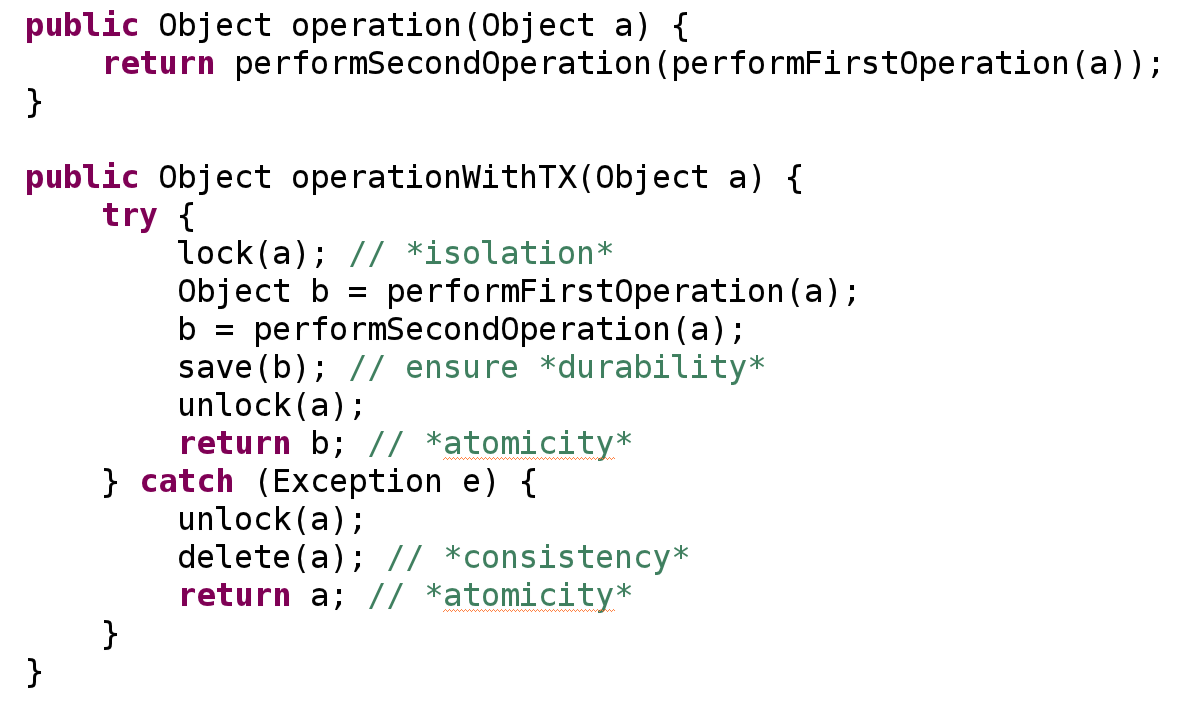
\includegraphics[scale=0.4]{img/transaction-cost.png}
      \caption{Coût en performance d'une transaction}
      \label{tx-cost}
    \end{center}
  \end{figure}

  \paragraph{} Le pseudo code présenté \ref{tx-cost} (page \pageref{tx-cost} n'est fourni
  qu'à titre d'exemple pédagogique. Lors de la mise en place de transaction au sein d'une
  application, le conteneur d'exécution, qu'il s'agisse d'une machine virtuelle ou du serveur
  d'application, fournit une API appropriée.

  % TODO Utilisé l'API et montrer les capacités de monitoring associé ?
}

\ifslide{
  \begin{frame}{Coût en performance d'une transaction}
   \begin{center}
     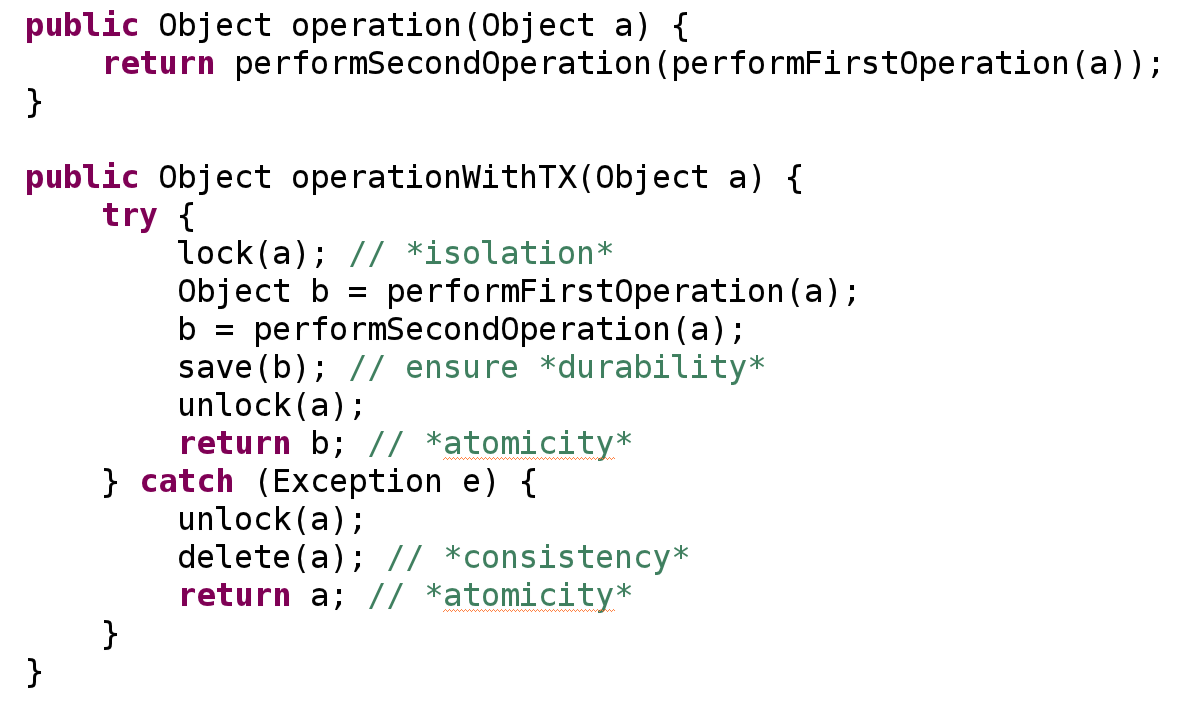
\includegraphics[scale=0.25]{img/transaction-cost.png}
   \end{center}
  \end{frame}
}

\ifbook{
  \mysubsubsection{Être (transactionnelle) ou ne pas être (transactionnel) ?}

  \paragraph{} Il est donc bien important, lors de la conception d'une application, de bien
  réfléchir à la nécessité ou non d'utiliser des transactions. Une preuve très flagrante de ceci est
  l'émergence des bases de données non transactionnel.

  \paragraph{} Avec l'augmentation des applications "web", mais surtout de leurs nombres
  d'utilisateurs, les bases de données relationnelles deviennent généralement le goulot
  d'étranglement. Comme évoqué précédemment, chaque requête vers ces base de données sont en effet
  des transactions exigeant, dans chaque tiers, un certains travail supplémentaire. En supprimant
  l'aspect transactionnel des échanges entres l'application et la source de données, ces bases de
  données offrent de bien meilleur performance.

  \paragraph{} Bien évidement, on s'expose aussi à des nombreux problèmes de corruption ou pertes de
  données, mais, il existe des applications où ce genre de situation est plus supportable qu'une
  perte de performance.

  \paragraph{} Par exemple, pour un jeu en ligne, que le tableau donnant la liste des 10 dernières
  meilleurs scores ne soit pas toujours cohérent et qu'il soit même parfois corrompu n'est pas un
  réel problème. A l'inverse, un le jeu qui devient trop lent, juste parce que les accès au tableau
  des meilleurs scores ralentit l'application, est un réel problème.
}

\newpage
\mysubsection{Cache}

\newcommand{\allcaches}[0]{
  \begin{itemize}
    \item cache DNS
    \item cache du navigateur
    \item cache HTTP
    \item la session est un cache
    \item cache SQL %(Hibernate)
    \item cache applicatif
  \end{itemize}
}

\ifbook{
  \paragraph{} Cette dernière section s'attarde sur les nombreux caches auquel une application
  seront confronté par l'intermédiaire du \textit{Middleware} qu'elle utilisera. Comme nous allons
  le voir, les caches sont partout, posent parfois des problèmes et sont malheureusement (ou pas)
  indispensables.

  \mysubsubsection{Rôle d'un cache}

  \paragraph{} Le rôle d'un cache est en fait très simple: il s'agit de conserver une information "à
  porté de main", pour ne pas avoir à aller la recherche "plus loin", par la suite. Pour prendre un
  exemple trivial, un bricoleur du dimanche qui sort un pack de bière du frigo et les descend avec
  lui dans la cave, où il va travailler, se créer simplement un cache de bière\footnote{.. et
  probablement quelques problèmes de santé à la longue.}, pour ne pas avoir à retourner en chercher.

  \paragraph{} Et de la même manière que la bière de notre bricoleur du dimanche va refroidir, les
  informations placées dans un cache risquent de rapidement se retrouver dans un état incohérent
  avec la source de donnée. Un cache implique donc souvent de mettre en place une \textbf{stratégie
  d'éviction}, plus ou moins complexe, pour s'assurer que notre application ne manipule jamais de
  données périmées ou invalides.

  \paragraph{} En conclusion, mettre une donnée en cache une donnée consiste à la sauvegarder dans
  un système plus facilement accessible, ou plus performant, que la source de données d'où elle
  provient, permettant ainsi de rapidement la retrouver, et d'éviter d'effectuer de nouveau
  l'opération de récupération.

  \paragraph{Intérêt des caches} Le seul et unique intérêt du cache est la \textbf{performance} de
  l'application. Maintenant, il est important de réaliser qu'ils ne sont pour autant en aucun cas
  dispensable. Sans cache, la plupart des applications sont généralement tellement lente qu'elles
  deviennent simplement inutilisable.

  \paragraph{Contraintes associées} Les caches contenant des informations qui sont désynchronisés
  de la source de données, ils ont souvent tendance à cacher d'éventuel dysfonctionnement, de
  manière partielle ou non, rendant complexe leur résolution. En outre, la \textbf{stratégie de mise
  en cache} adoptée, comme celle d'\textbf{éviction} sont critiques pour le fonctionnement correcte
  de l'applicatif.

  \mysubsubsection{Où se situent les caches ?}

  \paragraph{} La réponse est un peu partout ! L'inventaire suivante présente les caches les plus
  usuels qu'une application "Web" sera naturellement amené à utiliser:

  \allcaches
}

\ifslide{
  \begin{frame}{Cache sind über alles}
    \begin{center}
      \begin{block}{Différents caches}
        \allcaches
      \end{block}
    \end{center}
  \end{frame}
}

\ifbook{
  \mysubsubsection{Niveau de cache}

  \paragraph{} Sans rentrer dans les détails les plus pointues sur la gestion de cache, on notera
  qu'il existe plusieurs niveau de cache. Ces derniers sont généralement consultés les uns après les
  autres, par ordre d'efficacité, jusqu'à que l'un d'eux soit en mesure de retourner l'information
  recherché ou, si aucun ne le peut, l'application se retourne vers la source de données.

  \paragraph{} Prenons un exemple concret de niveau de cache. Lorsqu'une application nécessite une
  information d'authentification, elle dispose généralement d'un jeton d'authentification. Si elle
  ne dispose pas de ce jeton en mémoire, elle consulte généralement le contenu de la session pour
  l'y retrouver. Si ce dernier est périmé ou absent, l'application effectue de nouveau
  l'authentification de l'utilisateur.

  \paragraph{} Dans cet exemple, la mémoire de l'application fait, en fait, office de cache de
  premier niveau, et la session de cache de second niveau.

  \mysubsubsection{Un exemple de stratégie de cache: le "long tail catalog"}

  \paragraph{} Pour illustrer notre propos sur l'importance des caches, étudions un cas classique
  des applications en ligne: le \textit{long tail catalog}. Ce scénario est simple, une boutique en
  ligne dispose d'un catalogue de taille N, où est N est beaucoup plus grand que la mémoire M,
  disponible pour l'application.

  \paragraph{} Compte tenu qu'il est relativement coûteux, en terme de performance, de retrouver les
  éléments du catalogue depuis la source de données, on optimise généralement le système en plaçant
  en cache, de taille N, les données les plus demandées.

  \paragraph{} Une implémentation simple, et élégante, consiste à placer toutes informations
  retrouvées depuis la source de données en cache, et lui associer une date de péremption (par
  exemple, une heure après sa mise en cache). À chaque fois que la donnée est retrouvé dans le
  cache, sa date de péremption est repoussée d'une heure.

  \paragraph{} Ainsi, après quelques heures d'exécutions, le cache de l'application contiendra les
  N données les plus souvent demandées du catalogue complet, contenant M élément. Il est donc
  vraisemblable que la plupart des requêtes effectuées par les clients de la boutique en ligne, soit
  assez rapide.

  \paragraph{} Les requêtes marginales seront bien évidemment moins performantes, mais l'impact
  négatif, en terme de vente, sera bien moindre...
}

